
\documentclass[11pt]{article}
\usepackage[margin=2cm]{geometry}

% Core packages
\usepackage{amsmath,amssymb}
\usepackage{amsthm}
\usepackage{tikz}
\usepackage{tikz-cd}
\usepackage{multicol}
\usepackage{float}
\usepackage[colorlinks=true,linkcolor=blue,citecolor=blue,urlcolor=blue,bookmarksopen=true,bookmarksnumbered=true,pdfpagemode=UseOutlines,linktoc=all]{hyperref}

% Paragraphs
\setlength{\parindent}{0pt}
\setlength{\parskip}{1\baselineskip}

\newtheorem{theorem}{Theorem}[section]
\newtheorem{lemma}[theorem]{Lemma}
\newtheorem{corollary}[theorem]{Corollary}
\newtheorem{proposition}[theorem]{Proposition}

\newtheorem{conjecture}[theorem]{Conjecture}
\theoremstyle{definition}
\newtheorem{definition}[theorem]{Definition}
\newtheorem{example}[theorem]{Example}

\title{Analytic Number Theory}
\author{Daniel Soto Villada}
\date{}

\begin{document}
\maketitle

\begin{center}
Classroom: 4-218\\
Thursday, 14:00--16:00
\end{center}

Initial proposal of the topics to be covered, in order.

\begingroup
\small
\setlength{\parskip}{0pt}
\tableofcontents
\endgroup
\clearpage

\section{Set Theory}

This section introduces basic set notation, relations, and equivalence classes. The presentation follows the treatment of these foundations in \cite[Chapter 1, especially Section 1.6]{Berberian1998-qc}.

\subsection{Basic Set Notation}

\begin{definition}[Subset and equality]
Let $A$ and $B$ be sets. We say that $A$ is a subset of $B$, and write $A\subseteq B$, if every element of $A$ is also an element of $B$. The sets are equal if they have exactly the same elements; equivalently, $A=B$ if and only if $A\subseteq B$ and $B\subseteq A$.
\end{definition}

\begin{proposition}
For any sets $A$ and $B$, $A=B$ if and only if each is a subset of the other.
\end{proposition}

\begin{proof}
If $A=B$, then they have the same elements, so $A\subseteq B$ and $B\subseteq A$. Conversely, if both inclusions hold, an element belongs to $A$ exactly when it belongs to $B$. Thus the sets have the same elements and are equal.
\end{proof}

\begin{definition}[Set operations]
For sets $A$ and $B$, their union and intersection are
\[
 A\cup B=\{x:x\in A\text{ or }x\in B\},\qquad
 A\cap B=\{x:x\in A\text{ and }x\in B\}.
\]
Their difference is $A\setminus B=\{x\in A:x\notin B\}$. If a universal set $X$ is fixed and $A\subseteq X$, the complement of $A$ in $X$ is $X\setminus A$.
\end{definition}

\begin{definition}[Cartesian product]
For sets $X$ and $Y$, the Cartesian product is the set
\[
 X\times Y=\{(x,y):x\in X,\ y\in Y\}
\]
of ordered pairs.
\end{definition}

\subsection{Relations and Equivalence Relations}

\begin{definition}[Relation]
A relation from a set $X$ to a set $Y$ is a subset $R\subseteq X\times Y$. A relation in $X$ is a relation from $X$ to itself. We write $x\,R\,y$ when $(x,y)\in R$.
\end{definition}

\begin{definition}[Equivalence relation]
A relation $\sim$ in a set $X$ is an equivalence relation if, for all $x,y,z\in X$, it is:
\begin{enumerate}
    \item reflexive: $x\sim x$;
    \item symmetric: if $x\sim y$, then $y\sim x$;
    \item transitive: if $x\sim y$ and $y\sim z$, then $x\sim z$.
\end{enumerate}
\end{definition}

\begin{example}[Equality of function values]
Let $f:X\to Y$ be a function. Define $x\sim y$ when $f(x)=f(y)$. This is an equivalence relation: equality is reflexive, symmetric, and transitive, so the same three properties hold for $\sim$.
\end{example}

\subsection{Equivalence Classes and Quotient Sets}

\begin{definition}[Equivalence class]
If $\sim$ is an equivalence relation on $X$ and $x\in X$, the equivalence class of $x$ is
\[
 [x]=\{y\in X:y\sim x\}.
\]
The quotient set is the set of all equivalence classes,
\[
 X/{\sim}=\{[x]:x\in X\}.
\]
\end{definition}

\begin{theorem}[Equivalence classes partition a set]
Let $\sim$ be an equivalence relation on $X$. Every element of $X$ belongs to an equivalence class, and any two equivalence classes are either equal or disjoint.
\end{theorem}

\begin{proof}
Reflexivity gives $x\sim x$, so $x\in[x]$ for each $x\in X$. Now suppose $[x]\cap[y]\ne\varnothing$ and choose $z\in[x]\cap[y]$. Then $z\sim x$ and $z\sim y$. By symmetry and transitivity, $x\sim y$. If $t\in[x]$, then $t\sim x$ and $x\sim y$, so $t\sim y$ and $t\in[y]$. Thus $[x]\subseteq[y]$; the same argument with $x$ and $y$ interchanged gives $[y]\subseteq[x]$. Hence $[x]=[y]$.
\end{proof}

\begin{corollary}
Two elements $x,y\in X$ are equivalent if and only if their equivalence classes are equal.
\end{corollary}

\begin{proof}
If $x\sim y$, transitivity and symmetry show that an element belongs to $[x]$ exactly when it belongs to $[y]$, so $[x]=[y]$. Conversely, if $[x]=[y]$, then $x\in[x]=[y]$, which means $x\sim y$.
\end{proof}

\begin{example}[Integers modulo $m$]
Fix a positive integer $m$. On $\mathbb{Z}$, define $a\sim b$ if $m$ divides $a-b$. This is an equivalence relation: $m$ divides $a-a=0$; divisibility of $a-b$ implies divisibility of $b-a$; and if $m$ divides both $a-b$ and $b-c$, it divides their sum $a-c$. Its equivalence classes collect the integers with the same remainder upon division by $m$.
\end{example}
Taking $m=3$ gives a concrete partition of $\mathbb{Z}$. Each row below displays representative integers from one equivalence class; the ellipses indicate that each class continues indefinitely in both directions.
\[
 [r]_3=\{r+3k:k\in\mathbb{Z}\},\qquad r\in\{0,1,2\},
 \qquad
 \mathbb{Z}=[0]_3\,\dot\cup\,[1]_3\,\dot\cup\,[2]_3.
\]

\begin{figure}[htbp]
\centering
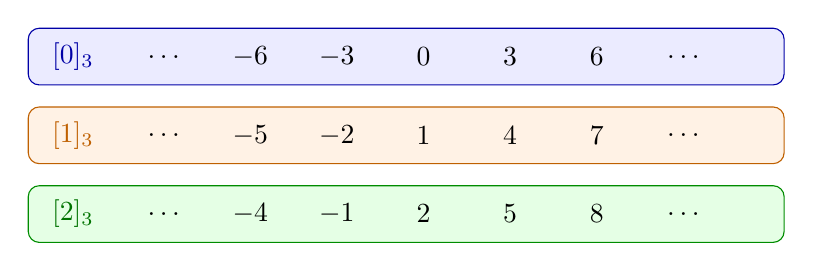
\begin{tikzpicture}[x=1.1cm,y=1cm]
    \node[draw=blue!65!black,fill=blue!8,rounded corners,minimum width=9.6cm,minimum height=0.72cm,inner sep=2pt] at (4.8,2) {};
    \node[draw=orange!75!black,fill=orange!10,rounded corners,minimum width=9.6cm,minimum height=0.72cm,inner sep=2pt] at (4.8,1) {};
    \node[draw=green!55!black,fill=green!10,rounded corners,minimum width=9.6cm,minimum height=0.72cm,inner sep=2pt] at (4.8,0) {};

    \node[anchor=west,text=blue!65!black,font=\bfseries] at (0.6,2) {$[0]_3$};
    \node[anchor=west,text=orange!75!black,font=\bfseries] at (0.6,1) {$[1]_3$};
    \node[anchor=west,text=green!45!black,font=\bfseries] at (0.6,0) {$[2]_3$};

    \foreach \x/\value in {2.0/{\ldots},3.0/{-6},4.0/{-3},5.0/{0},6.0/{3},7.0/{6},8.0/{\ldots}} {
        \node at (\x,2) {$\value$};
    }
    \foreach \x/\value in {2.0/{\ldots},3.0/{-5},4.0/{-2},5.0/{1},6.0/{4},7.0/{7},8.0/{\ldots}} {
        \node at (\x,1) {$\value$};
    }
    \foreach \x/\value in {2.0/{\ldots},3.0/{-4},4.0/{-1},5.0/{2},6.0/{5},7.0/{8},8.0/{\ldots}} {
        \node at (\x,0) {$\value$};
    }
\end{tikzpicture}
\caption{The equivalence classes of integers modulo $3$. Each row is one class; distinct rows are disjoint and together contain all integers.}
\label{fig:equivalence-classes-mod-3}
\end{figure}
\section{Real Analysis}

This section develops the real-sequence notions of convergence and limit superior and inferior, together with the basic definition of a series. These topics follow the treatment of the real numbers and convergence in \cite[Chapter 1, Sections 1.8 and 1.16]{Berberian1998-qc}.

\subsection{Sequences and Convergence}

\begin{definition}[Sequence]
A real sequence is a function $a:\mathbb{N}\to\mathbb{R}$. Its value at $n$ is denoted by $a_n$, and the sequence is written $(a_n)_{n\geq 1}$ or simply $(a_n)$.
\end{definition}

\begin{definition}[Convergence]
A sequence $(a_n)$ converges to $L\in\mathbb{R}$ if for every $\varepsilon>0$ there is an integer $N$ such that
\[
 n\geq N\quad\Longrightarrow\quad |a_n-L|<\varepsilon.
\]
In this case, $L$ is called the limit of the sequence and we write $a_n\to L$.
\end{definition}

\begin{figure}[htbp]
\centering
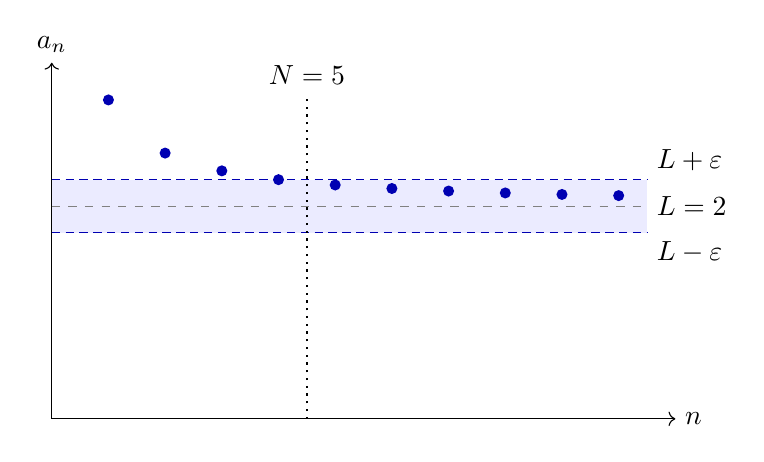
\begin{tikzpicture}[x=0.72cm,y=1.35cm]
    \fill[blue!8] (0,1.75) rectangle (10.5,2.25);
    \draw[->] (0,0) -- (11,0) node[right] {$n$};
    \draw[->] (0,0) -- (0,3.35) node[above] {$a_n$};
    \draw[dashed,gray] (0,2) -- (10.5,2) node[right,black] {$L=2$};
    \draw[densely dashed,blue!70!black] (0,2.25) -- (10.5,2.25) node[right,black,yshift=7pt] {$L+\varepsilon$};
    \draw[densely dashed,blue!70!black] (0,1.75) -- (10.5,1.75) node[right,black,yshift=-7pt] {$L-\varepsilon$};
    \draw[dotted,thick] (4.5,0) -- (4.5,3.05) node[above] {$N=5$};
    \foreach \n/\y in {1/3,2/2.5,3/2.333,4/2.25,5/2.2,6/2.167,7/2.143,8/2.125,9/2.111,10/2.1} {
        \fill[blue!70!black] (\n,\y) circle (2pt);
    }
\end{tikzpicture}
\caption{The sequence $a_n=2+1/n$ approaches $L=2$. For $\varepsilon=0.25$, all terms with $n\geq5$ lie inside the shaded band.}
\label{fig:sequence-convergence}
\end{figure}

\begin{theorem}[Uniqueness of limits]
A convergent real sequence has exactly one limit.
\end{theorem}

\begin{proof}
Suppose $a_n\to L$ and $a_n\to M$. For any $\varepsilon>0$, choose an index after which both $|a_n-L|<\varepsilon/2$ and $|a_n-M|<\varepsilon/2$. The triangle inequality gives
\[
 |L-M|\leq |L-a_n|+|a_n-M|<\varepsilon.
\]
Since this holds for every positive $\varepsilon$, $|L-M|=0$ and hence $L=M$.
\end{proof}

\begin{theorem}[Convergent sequences are bounded]
Every convergent real sequence is bounded.
\end{theorem}

\begin{proof}
Let $a_n\to L$. Taking $\varepsilon=1$, there is an index $N$ such that $|a_n-L|<1$ for every $n\geq N$. Thus $|a_n|<|L|+1$ for all such $n$. The finitely many terms $a_1,\ldots,a_{N-1}$ are also bounded, so the entire sequence is bounded.
\end{proof}

\clearpage

\begin{definition}[Cauchy sequence]
A real sequence $(a_n)$ is a Cauchy sequence if for every $\varepsilon>0$ there is an integer $N$ such that
\[
 m,n\geq N\quad\Longrightarrow\quad |a_m-a_n|<\varepsilon.
\]
\end{definition}

\begin{figure}[H]
\centering
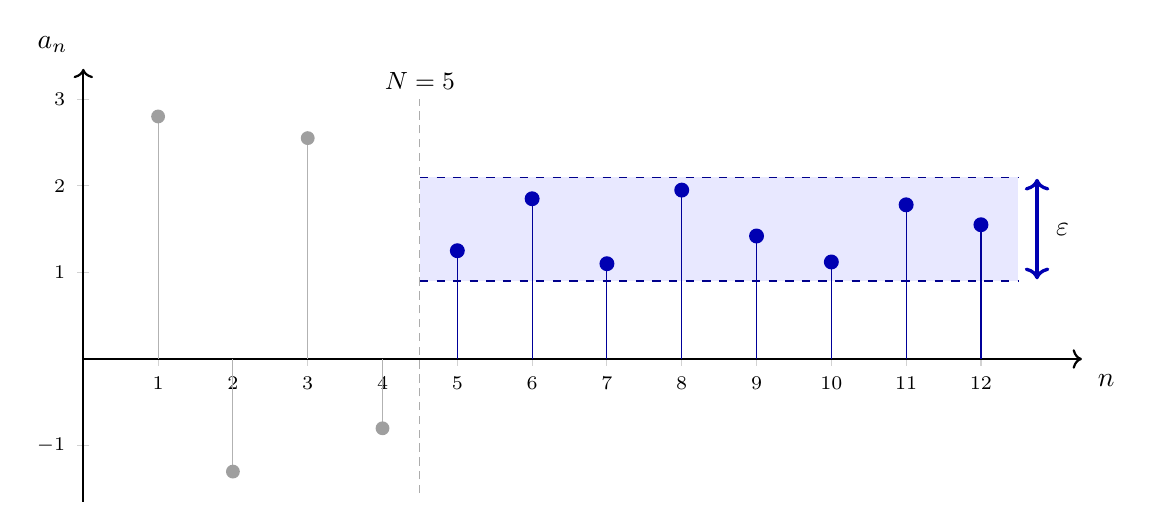
\begin{tikzpicture}[x=0.95cm,y=1.1cm]
    \path[fill=blue!9] (4.5,0.9) rectangle (12.5,2.1);
    \draw[blue!55!black,dashed] (4.5,0.9) -- (12.5,0.9);
    \draw[blue!55!black,dashed] (4.5,2.1) -- (12.5,2.1);
    \draw[gray!65,densely dashed] (4.5,-1.55) -- (4.5,3.0);
    \node[above,font=\small] at (4.5,3.0) {$N=5$};
    \draw[<->,very thick,blue!70!black] (12.75,0.92) -- (12.75,2.08)
        node[midway,right=3pt,black] {$\varepsilon$};

    \foreach \n in {1,...,12} {
        \draw[gray!35] (\n,0) -- (\n,-0.08);
        \node[below=3pt,font=\scriptsize] at (\n,0) {$\n$};
    }
    \foreach \y in {-1,1,2,3} {
        \draw[gray!35] (0.08,\y) -- (-0.08,\y);
        \node[left=3pt,font=\scriptsize] at (0,\y) {$\y$};
    }
    \draw[->,thick] (0,0) -- (13.35,0) node[below right=2pt] {$n$};
    \draw[->,thick] (0,-1.65) -- (0,3.35) node[above left=2pt] {$a_n$};

    \foreach \n/\value in {1/2.8,2/-1.3,3/2.55,4/-0.8} {
        \draw[gray!60] (\n,0) -- (\n,\value);
        \fill[gray!75] (\n,\value) circle (2.5pt);
    }
    \foreach \n/\value in {5/1.25,6/1.85,7/1.1,8/1.95,9/1.42,10/1.12,11/1.78,12/1.55} {
        \draw[blue!60!black] (\n,0) -- (\n,\value);
        \fill[blue!70!black] (\n,\value) circle (2.7pt);
    }
\end{tikzpicture}
\caption{Illustration of the Cauchy condition for a chosen $\varepsilon$: from $N=5$ onward, all plotted terms lie strictly between two levels separated by $\varepsilon$, so any two tail terms differ by less than $\varepsilon$.}
\label{fig:cauchy-sequence-tail}
\end{figure}

\begin{proposition}
Every convergent real sequence is a Cauchy sequence.
\end{proposition}

\begin{proof}
Suppose $a_n\to L$. Given $\varepsilon>0$, choose $N$ such that $|a_n-L|<\varepsilon/2$ for every $n\geq N$. If $m,n\geq N$, then
\[
 |a_m-a_n|\leq |a_m-L|+|a_n-L|<\varepsilon.
\]
Therefore $(a_n)$ is Cauchy.
\end{proof}

\subsection{Limit Superior and Limit Inferior}

For a bounded real sequence, each tail has a supremum and an infimum. The supremum of the tails decreases as the starting index increases, while the infimum of the tails increases.

\begin{definition}[Limit superior and limit inferior]
For a bounded real sequence $(a_n)$, define
\[
 \limsup_{n\to\infty}a_n=\inf_{N\geq1}\sup_{n\geq N}a_n,
 \qquad
 \liminf_{n\to\infty}a_n=\sup_{N\geq1}\inf_{n\geq N}a_n.
\]
\end{definition}

\begin{theorem}
For every bounded real sequence $(a_n)$,
\[
 \liminf_{n\to\infty}a_n\leq\limsup_{n\to\infty}a_n.
\]
Moreover, $(a_n)$ converges if and only if these two quantities are equal; when they are equal, their common value is the limit of $(a_n)$.
\end{theorem}

\begin{proof}
For any two indices $M,N$, the tails beginning at $M$ and $N$ have a common term $a_k$ when $k\geq\max\{M,N\}$. Consequently,
\[
 \inf_{n\geq M}a_n\leq a_k\leq\sup_{n\geq N}a_n.
\]
Taking the supremum over $M$ on the left and the infimum over $N$ on the right proves the inequality.

If $a_n\to L$, then for every $\varepsilon>0$ all sufficiently late terms lie between $L-\varepsilon$ and $L+\varepsilon$. The tail infima and suprema, and therefore their respective limits, lie in the same interval. Since this holds for every $\varepsilon>0$, both are $L$.

Conversely, suppose both quantities equal $L$. For any $\varepsilon>0$, the definition of the infimum of the tail suprema gives an index $N_1$ for which $\sup_{n\geq N_1}a_n<L+\varepsilon$. The definition of the supremum of the tail infima gives an index $N_2$ for which $\inf_{n\geq N_2}a_n>L-\varepsilon$. For $n\geq\max\{N_1,N_2\}$, these bounds imply $L-\varepsilon<a_n<L+\varepsilon$. Hence $a_n\to L$.
\end{proof}

\begin{figure}[htbp]
\centering
\begin{tikzpicture}[x=0.62cm,y=1.15cm]
    \draw[->] (0,0) -- (13,0) node[right] {$n$};
    \draw[->] (0,-1.25) -- (0,1.75) node[above] {$a_n$};
    \draw[dashed,red!70!black] (0,1) -- (12.5,1) node[right,black] {$\limsup a_n=1$};
    \draw[dashed,blue!70!black] (0,-1) -- (12.5,-1) node[right,black] {$\liminf a_n=-1$};
    \foreach \n/\y in {1/0,2/1.5,3/-0.667,4/1.25,5/-0.8,6/1.167,7/-0.857,8/1.125,9/-0.889,10/1.1,11/-0.909,12/1.083} {
        \draw[gray!65] (\n,0) -- (\n,\y);
        \fill[black] (\n,\y) circle (2pt);
    }
\end{tikzpicture}
\caption{For $a_n=(-1)^n+1/n$, the even and odd subsequences approach $1$ and $-1$, respectively.}
\label{fig:limsup-liminf}
\end{figure}

\subsection{Series}

\begin{definition}[Series and partial sums]
Given a real sequence $(a_n)$, its $N$th partial sum is
\[
 S_N=\sum_{n=1}^{N}a_n.
\]
The series $\sum_{n=1}^{\infty}a_n$ converges to $S$ if the sequence of partial sums $(S_N)$ converges to $S$. Otherwise, the series diverges.
\end{definition}

\begin{figure}[htbp]
\centering
\begin{tikzpicture}[x=0.78cm,y=3.0cm]
    \draw[->] (0,0) -- (8,0) node[right] {$N$};
    \draw[->] (0,0) -- (0,1.18) node[above] {$S_N$};
    \draw[dashed,red!70!black] (0,1) -- (7.6,1) node[right,black] {$S=1$};
    \foreach \n/\s in {1/0.5,2/0.75,3/0.875,4/0.9375,5/0.96875,6/0.984375,7/0.9921875} {
        \draw[gray!65] (\n,0) -- (\n,\s);
        \fill[blue!70!black] (\n,\s) circle (2pt);
    }
\end{tikzpicture}
\caption{The partial sums $S_N=\sum_{n=1}^{N}2^{-n}=1-2^{-N}$ approach the sum $1$.}
\label{fig:series-partial-sums}
\end{figure}

\begin{theorem}[Necessary condition for convergence]
If $\sum_{n=1}^{\infty}a_n$ converges, then $a_n\to0$.
\end{theorem}

\begin{proof}
Let $S_N=\sum_{n=1}^{N}a_n$ and suppose $S_N\to S$. For $n\geq2$, $a_n=S_n-S_{n-1}$. Both partial-sum sequences on the right tend to $S$, so
\[
 a_n=S_n-S_{n-1}\longrightarrow S-S=0.
\]
\end{proof}

\begin{example}[Geometric series]
For a real number $r$ with $|r|<1$, the finite partial sums satisfy
\[
 \sum_{n=0}^{N}r^n=\frac{1-r^{N+1}}{1-r}.
\]
Since $r^{N+1}\to0$, the geometric series converges and
\[
 \sum_{n=0}^{\infty}r^n=\frac{1}{1-r}.
\]
\end{example}
\section{Number Theory}

This section develops the elementary arithmetic of the integers that underlies analytic number theory. Its organization follows the treatment of divisibility, prime factorization, arithmetic functions, and congruences in Apostol \cite[Chapters 1, 2, and 5]{Apostol1976-xj}. The discussion of residue classes also prepares the way for Dirichlet characters and $L$-functions, as in the course outline in \textit{Guia2}.

\subsection{Divisibility and the Greatest Common Divisor}

\begin{definition}[Divisibility]
For integers $a$ and $b$, with $a\ne 0$, we say that $a$ divides $b$, and write $a\mid b$, if there is an integer $q$ such that $b=aq$. In this case, $a$ is a divisor of $b$ and $b$ is a multiple of $a$.
\end{definition}

\begin{theorem}[Division algorithm]
For every integer $a$ and positive integer $b$, there are unique integers $q$ and $r$ such that
\[
 a=bq+r,\qquad 0\leq r<b.
\]
\end{theorem}

\begin{definition}[Greatest common divisor]
For integers $a$ and $b$ that are not both zero, the greatest common divisor $\gcd(a,b)$ is the unique positive integer $d$ that divides both $a$ and $b$ and is divisible by every common divisor of $a$ and $b$.
\end{definition}

\begin{theorem}[Euclidean algorithm and Bézout's identity]
For positive integers $a$ and $b$, repeated application of the division algorithm gives the Euclidean algorithm: divide successively, using each nonzero remainder as the next divisor. The last nonzero remainder is $\gcd(a,b)$. More generally, for integers $a,b$ that are not both zero, there exist integers $x,y$ such that
\[
 \gcd(a,b)=ax+by.
\]
\end{theorem}

\begin{proof}
At each division step, $r_{j-1}=q_jr_j+r_{j+1}$. A common divisor of $r_{j-1}$ and $r_j$ divides $r_{j+1}$, and a common divisor of $r_j$ and $r_{j+1}$ divides $r_{j-1}$. Thus consecutive pairs have the same common divisors, so the last nonzero remainder is the greatest common divisor. The remainders are integer linear combinations of the initial pair, by repeated substitution in the division equations. Consequently, the last nonzero remainder has the form $ax+by$. For integers of arbitrary sign, apply the algorithm to $|a|$ and $|b|$ and adjust the signs of the resulting coefficients; when one integer is zero, the identity follows directly.
\end{proof}

\begin{example}[Computing a greatest common divisor]
Applying the Euclidean algorithm gives
\begin{align*}
252&=1\cdot198+54,\\
198&=3\cdot54+36,\\
54&=1\cdot36+18,\\
36&=2\cdot18.
\end{align*}
Therefore, $\gcd(252,198)=18$. Back-substitution gives $18=4\cdot252-5\cdot198$, illustrating Bézout's identity.
\end{example}

\subsection{Prime Numbers and Unique Factorization}

\begin{definition}[Prime number]
An integer $p>1$ is prime if its only positive divisors are $1$ and $p$. An integer greater than $1$ that is not prime is composite.
\end{definition}

\begin{theorem}[Fundamental theorem of arithmetic]
Every integer $n>1$ is a product of primes, and this factorization is unique up to the order of its factors. Equivalently, it can be written uniquely as
\[
 n=\prod_{j=1}^{k}p_j^{\alpha_j},
\]
where $p_1<\cdots<p_k$ are primes and each $\alpha_j$ is a positive integer.
\end{theorem}

\begin{theorem}[Infinitude of primes]
There are infinitely many prime numbers.
\end{theorem}

\begin{proof}
Suppose that the complete list of primes were $p_1,\ldots,p_k$. The integer $N=p_1p_2\cdots p_k+1$ is greater than $1$, so it has a prime divisor. None of $p_1,\ldots,p_k$ divides $N$, since each leaves remainder $1$ upon division into $N$. This contradicts the assumption that the list contained every prime.
\end{proof}

\subsection{Congruences and Residue Classes}

\begin{definition}[Congruence]
Let $m$ be a positive integer. Integers $a$ and $b$ are congruent modulo $m$, written
\[
 a\equiv b\pmod m,
\]
if $m\mid(a-b)$.
\end{definition}

Congruence modulo $m$ is an equivalence relation on $\mathbb{Z}$. The equivalence class of $a$ is
\[
 [a]_m=\{a+qm:q\in\mathbb{Z}\},
\]
and the set of residue classes is
\[
 \mathbb{Z}/m\mathbb{Z}=\{[0]_m,[1]_m,\ldots,[m-1]_m\}.
\]
Addition and multiplication of residue classes are defined by $[a]_m+[b]_m=[a+b]_m$ and $[a]_m[b]_m=[ab]_m$. These operations do not depend on the chosen representatives.

\begin{theorem}[Solvability of a linear congruence]
The congruence $ax\equiv b\pmod m$ has an integer solution $x$ if and only if $\gcd(a,m)\mid b$.
\end{theorem}

\begin{proof}
The congruence is equivalent to an equation $ax-b=km$ for some integer $k$, or $ax+(-k)m=b$. Every integer linear combination of $a$ and $m$ is divisible by $d=\gcd(a,m)$, so a solution requires $d\mid b$. Conversely, if $d\mid b$, Bézout's identity gives integers $u,v$ with $au+mv=d$. Multiplying by $b/d$ yields $a(u b/d)+m(v b/d)=b$, so $x=u b/d$ solves the congruence.
\end{proof}

\subsection{Units and Euler's Totient Function}

A residue class $[a]_m$ has a multiplicative inverse modulo $m$ precisely when $\gcd(a,m)=1$. These invertible classes form the group of units $(\mathbb{Z}/m\mathbb{Z})^\times$ under multiplication.

\begin{definition}[Euler's totient function]
For a positive integer $m$, Euler's totient function is
\[
 \varphi(m)=\#\{a:1\leq a\leq m,\ \gcd(a,m)=1\}.
\]
Thus $\varphi(m)$ is the number of invertible residue classes modulo $m$.
\end{definition}

\begin{theorem}[Euler's theorem]
If $\gcd(a,m)=1$, then
\[
 a^{\varphi(m)}\equiv1\pmod m.
\]
\end{theorem}

\begin{proof}
Multiplication by $[a]_m$ permutes the invertible residue classes modulo $m$. Multiplying all classes in this permutation gives
\[
 [a]_m^{\varphi(m)}\prod_{\substack{1\leq r\leq m\\\gcd(r,m)=1}}[r]_m
 =\prod_{\substack{1\leq r\leq m\\\gcd(r,m)=1}}[r]_m.
\]
The product on the right is invertible, so it can be cancelled, yielding the claimed congruence.
\end{proof}

\begin{example}[Residue classes modulo $5$]
The classes modulo $5$ are $[0]_5,[1]_5,[2]_5,[3]_5,[4]_5$. The invertible classes are $[1]_5,[2]_5,[3]_5,[4]_5$, so $\varphi(5)=4$. For example, Euler's theorem gives $2^4\equiv1\pmod5$.
\end{example}

\begin{example}[A fully worked application modulo $12$]
For $m=12$, the greatest common divisors of the integers from $1$ to $12$ with $12$, in order, are
\[
 \bigl(\gcd(1,12),\gcd(2,12),\ldots,\gcd(12,12)\bigr)
 =(1,2,3,4,1,6,1,4,3,2,1,12).
\]
Hence the integers in this range that are relatively prime to $12$ are exactly $1,5,7,11$, and the totient value is
\[
 \varphi(12)=\#\{r:1\leq r\leq12,\ \gcd(r,12)=1\}
 =\#\{1,5,7,11\}=4.
\]
Equivalently, since the numbers not relatively prime to $12$ are those divisible by $2$ or $3$, inclusion--exclusion gives
\[
 \varphi(12)=12-\frac{12}{2}-\frac{12}{3}+\frac{12}{6}=4.
\]
Now take $a=5$. Since $\gcd(5,12)=1$, Euler's theorem applies, with exponent $\varphi(12)=4$. Direct calculation verifies the conclusion:
\[
 5^{\varphi(12)}=5^4=(5^2)^2=25^2=625=52\cdot12+1,
 \qquad\text{so}\qquad 5^4\equiv1\pmod{12}.
\]
\end{example}

The unit classes and their multiplicative characters are the algebraic starting point for Dirichlet $L$-functions, developed in a later section and in the course guide \textit{Guia2}.

\subsection{Divisors and Abundant Numbers}

\begin{definition}[Sum-of-divisors function]
For a positive integer $n$, define
\[
 \sigma(n)=\sum_{d\mid n}d,
\]
the sum of all positive divisors of $n$.
\end{definition}

\begin{theorem}[Formula for the sum of divisors]
If $n=\prod_{j=1}^{k}p_j^{\alpha_j}$ is the prime factorization of $n$, then
\[
 \sigma(n)=\prod_{j=1}^{k}\left(1+p_j+p_j^2+\cdots+p_j^{\alpha_j}\right)
 =\prod_{j=1}^{k}\frac{p_j^{\alpha_j+1}-1}{p_j-1}.
\]
\end{theorem}

\begin{proof}
Every positive divisor of $n$ is obtained by choosing, independently for each prime $p_j$, an exponent from $0$ to $\alpha_j$. Summing the resulting products over all choices factors into the product of the geometric sums shown above.
\end{proof}

\begin{definition}[Abundant number]
A positive integer $n$ is abundant if the sum of its proper positive divisors is greater than $n$. Since the proper divisors omit $n$ itself, this is equivalent to $\sigma(n)>2n$.
\end{definition}

\begin{example}
The positive divisors of $12$ are $1,2,3,4,6,12$. Their sum is $\sigma(12)=28$, and the proper divisors sum to $1+2+3+4+6=16>12$. Thus $12$ is abundant.
\end{example}

\subsection{A First Look at the Distribution of Primes}

\begin{definition}[Prime-counting function]
For real $x\geq2$, let
\[
 \pi(x)=\#\{p\leq x:p\text{ is prime}\}.
\]
\end{definition}

\begin{theorem}[Prime number theorem]
\[
 \pi(x)\sim\frac{x}{\log x}\qquad(x\to\infty),
\]
\end{theorem}

Here $f(x)\sim g(x)$ means that $f(x)/g(x)\to1$. This asymptotic description is one of the central results of analytic number theory; its proof is deferred to the later study of prime distribution \cite[Chapter 4]{Apostol1976-xj}.
\begin{figure}[H]
\centering
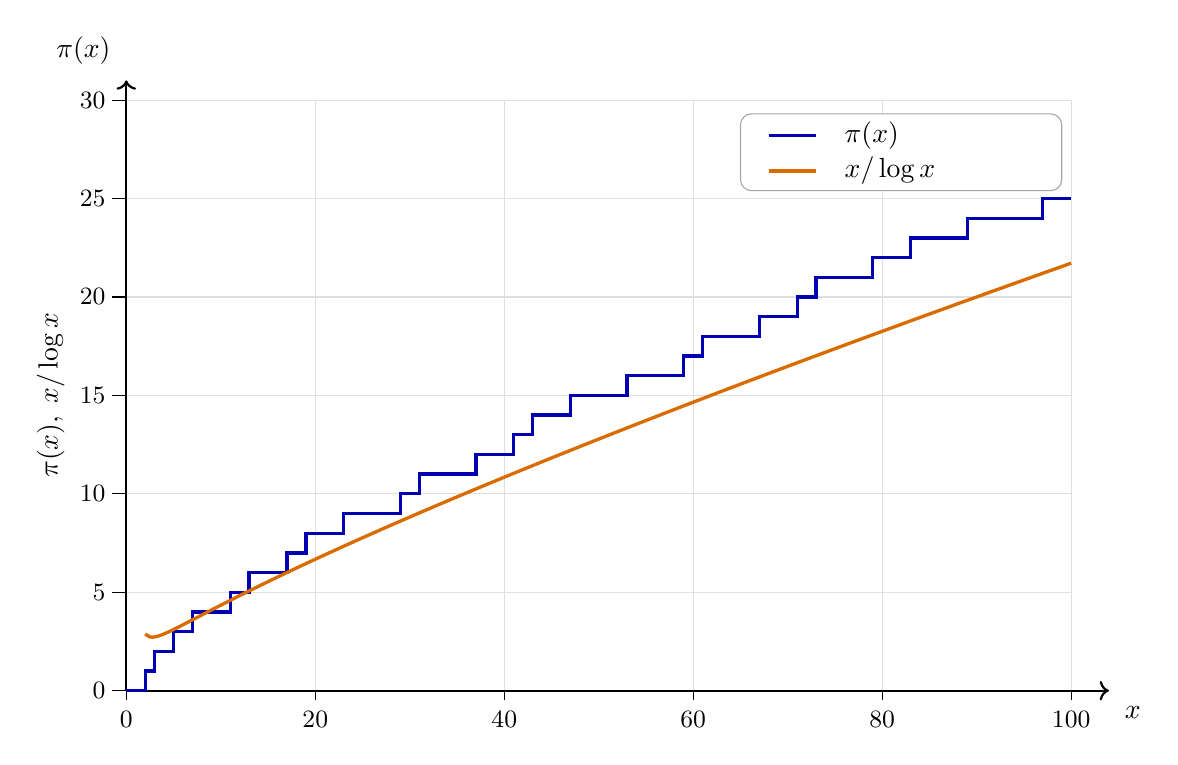
\begin{tikzpicture}[x=0.12cm,y=0.25cm]
    \foreach \x in {0,20,...,100} {
        \draw[gray!25,thin] (\x,0) -- (\x,30);
        \draw[black] (\x,0) -- (\x,-0.45);
        \node[below=4pt] at (\x,0) {\small \x};
    }
    \foreach \y in {0,5,...,30} {
        \draw[gray!25,thin] (0,\y) -- (100,\y);
        \draw[black] (0,\y) -- (-1.5,\y);
        \node[left=4pt] at (0,\y) {\small \y};
    }

    \draw[->,thick] (0,0) -- (104,0) node[below right=2pt] {$x$};
    \draw[->,thick] (0,0) -- (0,31) node[above left=2pt] {$\pi(x)$};
    \node[rotate=90] at (-8,15) {$\pi(x),\;x/\log x$};

    \draw[blue!70!black,very thick]
        (0,0) -- (2,0) -- (2,1) -- (3,1) -- (3,2) -- (5,2) -- (5,3)
        -- (7,3) -- (7,4) -- (11,4) -- (11,5) -- (13,5) -- (13,6)
        -- (17,6) -- (17,7) -- (19,7) -- (19,8) -- (23,8) -- (23,9)
        -- (29,9) -- (29,10) -- (31,10) -- (31,11) -- (37,11) -- (37,12)
        -- (41,12) -- (41,13) -- (43,13) -- (43,14) -- (47,14) -- (47,15)
        -- (53,15) -- (53,16) -- (59,16) -- (59,17) -- (61,17) -- (61,18)
        -- (67,18) -- (67,19) -- (71,19) -- (71,20) -- (73,20) -- (73,21)
        -- (79,21) -- (79,22) -- (83,22) -- (83,23) -- (89,23) -- (89,24)
        -- (97,24) -- (97,25) -- (100,25);

    \draw[orange!85!black,very thick,samples=200,domain=2:100,smooth,variable=\x]
        plot (\x,{\x/ln(\x)});

    \path[fill=white,draw=black!35,rounded corners] (65,25.4) rectangle (99,29.3);
    \draw[blue!70!black,very thick] (68,28.2) -- (73,28.2);
    \node[anchor=west] at (75,28.2) {$\pi(x)$};
    \draw[orange!85!black,very thick] (68,26.4) -- (73,26.4);
    \node[anchor=west] at (75,26.4) {$x/\log x$};
\end{tikzpicture}
\caption{The prime-counting function $\pi(x)$ and its asymptotic comparison $x/\log x$ on $2\leq x\leq100$.}
\label{fig:prime-number-theorem}
\end{figure}

The plot illustrates the prime number theorem on a finite interval; the asymptotic equivalence concerns the limit as $x\to\infty$ and is not established by this graph.
\section{Group Theory}

This section focuses on the group-theoretic tools needed for the course: in particular, the finite abelian groups of units modulo an integer and their multiplicative characters. The selection follows the introductory group material in Lee \cite[Chapters 3--5]{Lee2018-aa}.

\subsection{Groups and Groups of Units}

\begin{definition}[Group]
A group is a set $G$ equipped with a binary operation, written multiplicatively, such that:
\begin{enumerate}
    \item the operation is associative;
    \item there is an identity element $e\in G$ satisfying $eg=ge=g$ for every $g\in G$;
    \item every $g\in G$ has an inverse $g^{-1}\in G$ satisfying $gg^{-1}=g^{-1}g=e$.
\end{enumerate}
A group is abelian if $gh=hg$ for all $g,h\in G$.
\end{definition}

\begin{definition}[Subgroup]
A subset $H\subseteq G$ is a subgroup, written $H\leq G$, if it is a group under the operation inherited from $G$.
\end{definition}

The group relevant to Dirichlet characters is
\[
 U(m)=(\mathbb{Z}/m\mathbb{Z})^{\times},
\]
the group of invertible residue classes modulo $m$. As multiplication of residue classes is commutative, $U(m)$ is abelian. Its order is $\varphi(m)$, the number of residue classes relatively prime to $m$.

\begin{example}
For $m=5$, $U(5)=\{[1]_5,[2]_5,[3]_5,[4]_5\}$. Since
\[
 [2]_5^2=[4]_5,\qquad [2]_5^3=[3]_5,\qquad [2]_5^4=[1]_5,
\]
the group is cyclic, generated by $[2]_5$.
\end{example}

\subsection{Cosets, Orders, and Lagrange's Theorem}

\begin{definition}[Coset]
If $H\leq G$ and $g\in G$, the left coset of $H$ determined by $g$ is
\[
 gH=\{gh:h\in H\}.
\]
\end{definition}

The left cosets of $H$ partition $G$, and each has the same number of elements as $H$.

\begin{definition}[Order of an element]
For $g\in G$, the cyclic subgroup generated by $g$ is $\langle g\rangle=\{g^k:k\in\mathbb{Z}\}$. If this subgroup is finite, its number of elements is called the order of $g$ and is denoted $|g|$.
\end{definition}

\begin{theorem}[Lagrange's theorem]
If $G$ is a finite group and $H\leq G$, then
\[
 |G|=[G:H]|H|,
\]
where $[G:H]$ is the number of distinct left cosets of $H$ in $G$. In particular, the order of every element of $G$ divides $|G|$.
\end{theorem}

\begin{proof}
The left cosets partition $G$ and the map $h\mapsto gh$ is a bijection from $H$ to $gH$. Thus every coset has $|H|$ elements, and counting the elements of $G$ by cosets gives $|G|=[G:H]|H|$. For any $g\in G$, the powers of $g$ form the cyclic subgroup $\langle g\rangle$; applying the formula to this subgroup shows that the order of $g$ divides $|G|$.
\end{proof}

\subsection{Normal Subgroups and Quotient Groups}

\begin{definition}[Normal subgroup]
A subgroup $N\leq G$ is normal, written $N\trianglelefteq G$, if $gN=Ng$ for every $g\in G$.
\end{definition}

\begin{definition}[Quotient group]
If $N\trianglelefteq G$, the set of cosets
\[
G/N=\{gN:g\in G\}
\]
is a group under the operation $(gN)(hN)=(gh)N$. Normality ensures that this operation does not depend on the choice of coset representatives. The group is called the quotient group of $G$ by $N$.
\end{definition}

\begin{example}
The subgroup $m\mathbb{Z}$ is normal in the additive group $\mathbb{Z}$, and the quotient group $\mathbb{Z}/m\mathbb{Z}$ consists of the residue classes modulo $m$.
\end{example}

\subsection{Homomorphisms and the First Isomorphism Theorem}

\begin{definition}[Group homomorphism]
Let $G$ and $H$ be groups. A function $\varphi:G\to H$ is a group homomorphism if
\[
 \varphi(g_1g_2)=\varphi(g_1)\varphi(g_2)
 \qquad\text{for all }g_1,g_2\in G.
\]
Its kernel and image are
\[
 \ker\varphi=\{g\in G:\varphi(g)=e_H\},\qquad
 \operatorname{im}\varphi=\{\varphi(g):g\in G\}.
\]
An isomorphism is a bijective homomorphism; groups related by an isomorphism have the same group structure.
\end{definition}

If $N\trianglelefteq G$ and a homomorphism $\varphi:G\to H$ satisfies $N\subseteq\ker\varphi$, then $\varphi$ is constant on each coset of $N$. It therefore induces a homomorphism $\overline{\varphi}:G/N\to H$ defined by $\overline{\varphi}(gN)=\varphi(g)$, so that $\varphi=\overline{\varphi}\circ\pi$, where $\pi(g)=gN$ is the quotient map. The diagram illustrates this factorization:

\begin{figure}[H]
\centering
\begin{tikzcd}[column sep=large,row sep=large]
G \arrow[r,"\varphi"] \arrow[d,"\pi"'] & H \\
G/N \arrow[ur,"\overline{\varphi}"']
\end{tikzcd}
\caption{A homomorphism that is trivial on $N$ factors through the quotient $G/N$.}
\label{fig:quotient-factorization}
\end{figure}

\begin{theorem}[Kernel and image]
For a group homomorphism $\varphi:G\to H$, the kernel is a normal subgroup of $G$ and the image is a subgroup of $H$.
\end{theorem}

\begin{proof}
If $h_1=\varphi(g_1)$ and $h_2=\varphi(g_2)$ are in the image, then $h_1h_2^{-1}=\varphi(g_1g_2^{-1})$ is also in the image, so the image is a subgroup. Since $\varphi(e_G)=e_H$ and $\varphi(k_1k_2^{-1})=e_H$ whenever $k_1,k_2\in\ker\varphi$, the kernel is a subgroup. If $k\in\ker\varphi$ and $g\in G$, then
\[
 \varphi(gkg^{-1})=\varphi(g)\varphi(k)\varphi(g)^{-1}
 =\varphi(g)e_H\varphi(g)^{-1}=e_H.
\]
Thus $g(\ker\varphi)g^{-1}\subseteq\ker\varphi$; applying the same argument to $g^{-1}$ gives equality, so the kernel is normal.
\end{proof}

\begin{theorem}[First isomorphism theorem]
For every group homomorphism $\varphi:G\to H$,
\[
 G/\ker\varphi\cong\operatorname{im}\varphi.
\]
\end{theorem}

The theorem identifies the quotient by the kernel with the image. The diagram shows the quotient map, the induced isomorphism, and the inclusion of the image into $H$:

\begin{figure}[H]
\centering
\begin{tikzcd}[column sep=large,row sep=large]
G \arrow[r,"\varphi"] \arrow[d,"\pi"'] & H \\
G/\ker\varphi \arrow[r,"\overline{\varphi}"'] & \operatorname{im}\varphi \arrow[u,hook,"i"']
\end{tikzcd}
\caption{The first isomorphism theorem: $\overline{\varphi}$ is an isomorphism and $i$ is the inclusion.}
\label{fig:first-isomorphism}
\end{figure}

\begin{proof}
Define $\overline{\varphi}:G/\ker\varphi\to\operatorname{im}\varphi$ by $\overline{\varphi}(g\ker\varphi)=\varphi(g)$. If two cosets are equal, their representatives differ by an element of the kernel, so they have the same image; hence the map is well-defined. It is a homomorphism, is onto by the definition of the image, and is one-to-one because equal images imply that the representatives differ by an element of the kernel. Therefore it is an isomorphism.
\end{proof}

\subsection{Finite-Group Characters}

\begin{definition}[Multiplicative character]
A multiplicative character of a group $G$ is a homomorphism $\chi:G\to\mathbb{C}^{\times}$, where $\mathbb{C}^{\times}=\mathbb{C}\setminus\{0\}$ under multiplication. For a finite abelian group, its character group is
\[
 \widehat{G}=\operatorname{Hom}(G,\mathbb{C}^{\times}).
\]
The operation on $\widehat{G}$ is pointwise multiplication of characters.
\end{definition}

\begin{proposition}
If $G$ is finite and $\chi:G\to\mathbb{C}^{\times}$ is a character, then every value $\chi(g)$ is a root of unity.
\end{proposition}

\begin{proof}
For $g\in G$, let $r$ be its finite order. Then $g^r=e$, and the homomorphism property gives $\chi(g)^r=\chi(g^r)=\chi(e)=1$.
\end{proof}

For the course, take $G=U(m)$. A multiplicative character on $U(m)$ gives the values of a Dirichlet character on the invertible residue classes modulo $m$; it is extended to integers by assigning value $0$ to integers not relatively prime to $m$. For example, since $U(5)=\langle[2]_5\rangle$, one character is determined by $\chi([2]_5)=i$, yielding $\chi([1]_5)=1$, $\chi([2]_5)=i$, $\chi([4]_5)=-1$, and $\chi([3]_5)=-i$. These are the group-theoretic objects used to define Dirichlet $L$-functions.
\section{Complex Analysis}

This section introduces the complex-analytic tools needed later for the study of Dirichlet $L$-functions and zeta regularization: holomorphic and meromorphic functions, Cauchy's theorems, power series, analytic continuation, isolated singularities, and residues. The selection follows the treatment of analytic functions, complex integration, Taylor and Laurent series, and residue calculus in Kwok \cite[Chapters 2, 4--6]{Kwok2010}.

\subsection{Holomorphic, Entire, and Meromorphic Functions}

\begin{definition}[Domain]
A domain is a connected open subset of the complex plane $\mathbb{C}$.
\end{definition}

\begin{definition}[Holomorphic function]
Let $D$ be a domain. A function $f:D\to\mathbb{C}$ is holomorphic on $D$ if the complex derivative
\[
 f'(z)=\lim_{h\to 0}\frac{f(z+h)-f(z)}{h}
\]
exists for every $z\in D$.
\end{definition}

\begin{definition}[Entire function]
A function is entire if it is holomorphic on all of $\mathbb{C}$.
\end{definition}

\begin{example}
The functions $f(z)=z^n$ for each nonnegative integer $n$, and $f(z)=e^z$, are entire.
\end{example}

Holomorphicity is a strong condition: a holomorphic function has derivatives of every order and is locally represented by a convergent power series. The Cauchy integral formula below gives a central reason for these properties.

\subsection{Cauchy's Theorem and Integral Formula}

\begin{theorem}[Cauchy--Goursat theorem]
If $f$ is holomorphic on a domain containing a positively oriented simple closed contour $C$ and its interior, then
\[
 \oint_C f(z)\,dz=0.
\]
\end{theorem}

\begin{theorem}[Cauchy integral formula]
Let $C$ be a positively oriented simple closed contour, and suppose that $f$ is holomorphic on and inside $C$. For every point $a$ inside $C$,
\[
 f(a)=\frac{1}{2\pi i}\oint_C\frac{f(z)}{z-a}\,dz.
\]
Moreover, for every integer $n\geq 0$,
\[
 f^{(n)}(a)=\frac{n!}{2\pi i}\oint_C\frac{f(z)}{(z-a)^{n+1}}\,dz.
\]
\end{theorem}

\begin{figure}[H]
\centering
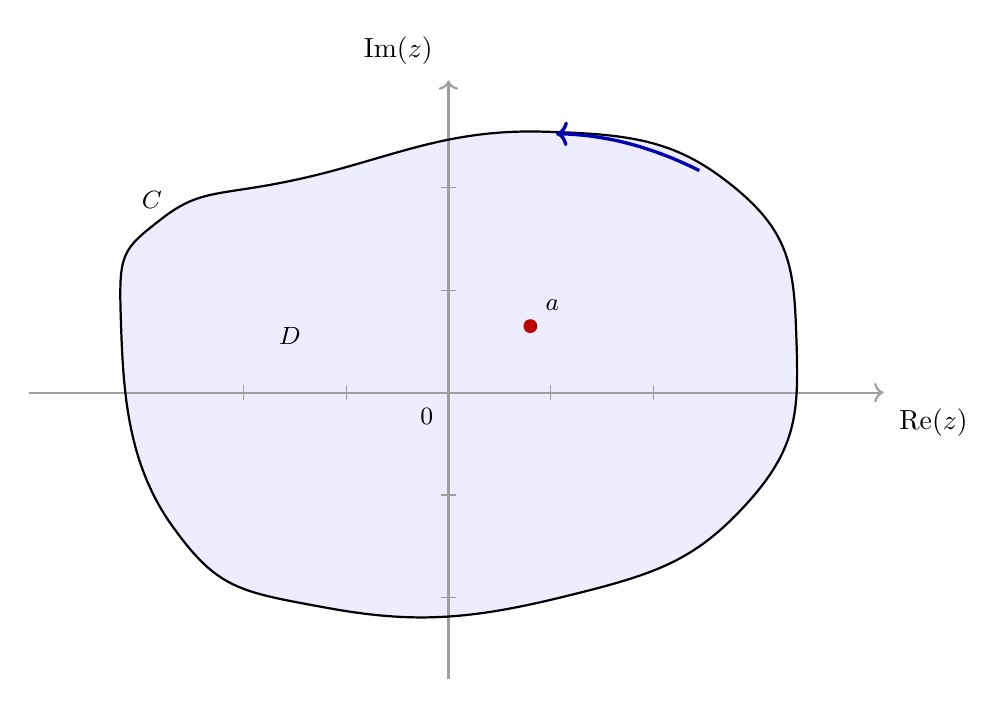
\begin{tikzpicture}[x=1.3cm,y=1.3cm]
    \path[fill=blue!7]
        plot[smooth cycle,tension=0.8] coordinates {
            (-3.2,0.7) (-2.7,-1.3) (-1.2,-2.1) (1.1,-2.0)
            (2.9,-1.1) (3.4,0.5) (2.8,2.0) (0.9,2.55)
            (-1.4,2.1) (-2.8,1.7)
        };
    \draw[->,gray!75,thick] (-4.1,0) -- (4.25,0)
        node[below right=2pt,black] {$\operatorname{Re}(z)$};
    \draw[->,gray!75,thick] (0,-2.8) -- (0,3.05)
        node[above left=2pt,black] {$\operatorname{Im}(z)$};
    \foreach \x in {-2,-1,1,2} {
        \draw[gray!75] (\x,0.07) -- (\x,-0.07);
    }
    \foreach \y in {-2,-1,1,2} {
        \draw[gray!75] (0.07,\y) -- (-0.07,\y);
    }
    \node[below left=2pt,font=\small] at (0,0) {$0$};
    \draw[thick]
        plot[smooth cycle,tension=0.8] coordinates {
            (-3.2,0.7) (-2.7,-1.3) (-1.2,-2.1) (1.1,-2.0)
            (2.9,-1.1) (3.4,0.5) (2.8,2.0) (0.9,2.55)
            (-1.4,2.1) (-2.8,1.7)
        };
    \draw[->,very thick,blue!70!black]
        (2.45,2.17) .. controls (1.95,2.42) and (1.5,2.52) .. (1.05,2.53);
    \node[above left=2pt,font=\small] at (-2.65,1.65) {$C$};
    \node[font=\small] at (-1.55,0.55) {$D$};
    \fill[red!75!black] (0.8,0.65) circle (2.5pt);
    \node[above right=2pt,font=\small] at (0.8,0.65) {$a$};
\end{tikzpicture}
\caption{A positively oriented simple closed contour $C$ enclosing the domain $D$ and the point $a$ in the complex plane.}
\label{fig:cauchy-contour-theorems}
\end{figure}

\begin{corollary}[Taylor expansion]
If $f$ is holomorphic on a disk centered at $a$, then in that disk it has the expansion
\[
 f(z)=\sum_{n=0}^{\infty}\frac{f^{(n)}(a)}{n!}(z-a)^n.
\]
\end{corollary}

\subsection{Taylor and Laurent Series}

Taylor series describe holomorphic functions near ordinary points. When a point is excluded from the domain, a series with both positive and negative powers is needed.

\begin{theorem}[Laurent expansion]
If $f$ is holomorphic on an annulus $r<|z-a|<R$, then there is a unique series
\[
 f(z)=\sum_{n=-\infty}^{\infty}c_n(z-a)^n
\]
that converges to $f$ throughout the annulus, uniformly on every compact subannulus. Its coefficients are
\[
 c_n=\frac{1}{2\pi i}\oint_{|z-a|=\rho}
 \frac{f(z)}{(z-a)^{n+1}}\,dz,
 \qquad r<\rho<R.
\]
\end{theorem}

The coefficient $c_{-1}$ is called the residue of $f$ at $a$, denoted by $\operatorname{Res}(f,a)$.

\subsection{Isolated Singularities and Residues}

\begin{definition}[Isolated singularity]
A point $a$ is an isolated singularity of $f$ if $f$ is holomorphic in some deleted neighborhood $0<|z-a|<r$ of $a$.
\end{definition}

The Laurent expansion classifies isolated singularities:
\begin{itemize}
    \item The singularity is removable if all coefficients with negative index vanish.
    \item It is a pole of order $m$ if $c_{-m}\neq 0$ and $c_n=0$ for every $n<-m$.
    \item It is essential if infinitely many coefficients with negative index are nonzero.
\end{itemize}

\begin{figure}[H]
\centering
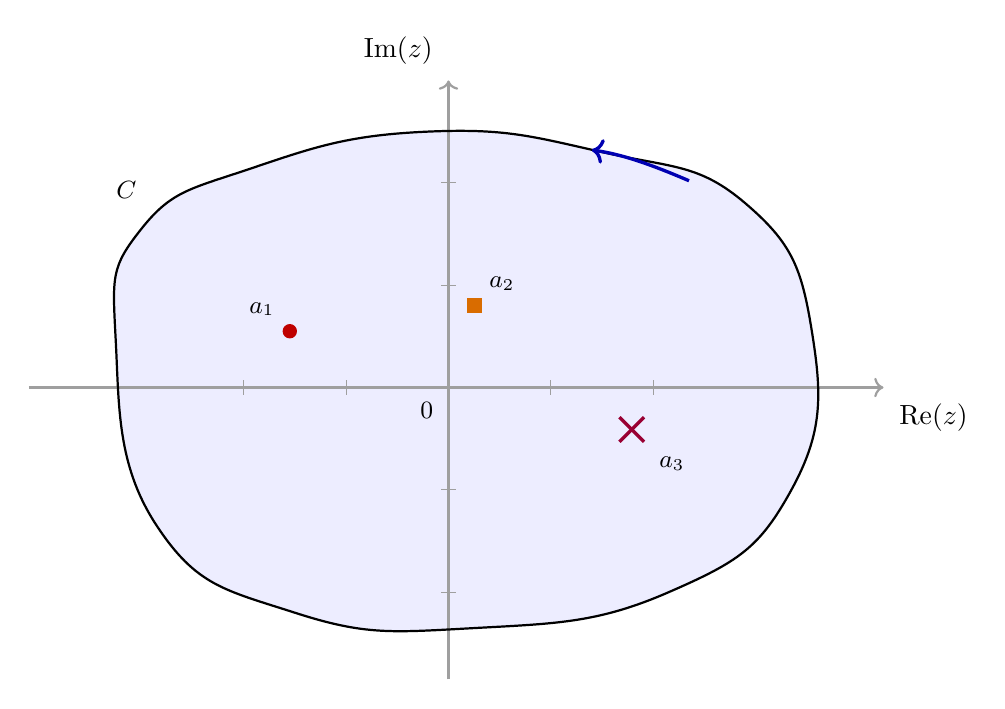
\begin{tikzpicture}[x=1.3cm,y=1.3cm]
    \path[fill=blue!7]
        plot[smooth cycle,tension=0.8] coordinates {
            (-3.25,0.45) (-2.85,-1.35) (-1.5,-2.2) (0.25,-2.35)
            (2.15,-2.0) (3.35,-1.0) (3.55,0.55) (2.9,1.8)
            (1.5,2.3) (-0.2,2.5) (-1.9,2.15) (-3.0,1.55)
        };
    \draw[->,gray!75,thick] (-4.1,0) -- (4.25,0)
        node[below right=2pt,black] {$\operatorname{Re}(z)$};
    \draw[->,gray!75,thick] (0,-2.85) -- (0,3.0)
        node[above left=2pt,black] {$\operatorname{Im}(z)$};
    \foreach \x in {-2,-1,1,2} {
        \draw[gray!75] (\x,0.07) -- (\x,-0.07);
    }
    \foreach \y in {-2,-1,1,2} {
        \draw[gray!75] (0.07,\y) -- (-0.07,\y);
    }
    \node[below left=2pt,font=\small] at (0,0) {$0$};
    \draw[thick]
        plot[smooth cycle,tension=0.8] coordinates {
            (-3.25,0.45) (-2.85,-1.35) (-1.5,-2.2) (0.25,-2.35)
            (2.15,-2.0) (3.35,-1.0) (3.55,0.55) (2.9,1.8)
            (1.5,2.3) (-0.2,2.5) (-1.9,2.15) (-3.0,1.55)
        };
    \draw[->,very thick,blue!70!black]
        (2.35,2.02) .. controls (2.0,2.17) and (1.7,2.28) .. (1.4,2.32);
    \node[above left=2pt,font=\small] at (-2.9,1.7) {$C$};

    \fill[red!75!black] (-1.55,0.55) circle (2.6pt);
    \node[above left=2pt,font=\small] at (-1.55,0.55) {$a_1$};
    \node[draw=orange!85!black,fill=orange!85!black,minimum size=5pt,inner sep=0pt]
        at (0.25,0.8) {};
    \node[above right=2pt,font=\small] at (0.25,0.8) {$a_2$};
    \draw[purple!80!black,line width=1.2pt] (1.67,-0.53) -- (1.91,-0.29);
    \draw[purple!80!black,line width=1.2pt] (1.67,-0.29) -- (1.91,-0.53);
    \node[below right=2pt,font=\small] at (1.91,-0.53) {$a_3$};
\end{tikzpicture}
\caption{The counterclockwise contour $C$ encloses isolated singularities: a simple pole at $a_1$ (circle), a pole of order two at $a_2$ (square), and an essential singularity at $a_3$ (cross).}
\label{fig:isolated-singularities-contour}
\end{figure}

\begin{definition}[Meromorphic function]
A function on a domain is meromorphic if it is holomorphic there except at isolated poles.
\end{definition}

\begin{example}
At $z=0$, the function $\sin z/z$ has a removable singularity, $1/z^2$ has a pole of order two, and $e^{1/z}$ has an essential singularity. These classifications follow from their Laurent expansions at the origin.
\end{example}

\begin{theorem}[Residue theorem]
Let $C$ be a positively oriented simple closed contour, and let $f$ be holomorphic on and inside $C$ except at finitely many isolated singularities $a_1,\ldots,a_k$ in its interior. Then
\[
 \oint_C f(z)\,dz=2\pi i\sum_{j=1}^{k}\operatorname{Res}(f,a_j).
\]
\end{theorem}

\begin{proof}
Remove small, disjoint disks around the singularities. The function is holomorphic on the remaining region, so Cauchy's theorem equates the integral over $C$ with the sum of the integrals over the small, positively oriented circles around each $a_j$. Integrating the Laurent series around each circle leaves only its $(z-a_j)^{-1}$ term, whose integral is $2\pi i\operatorname{Res}(f,a_j)$.
\end{proof}

\begin{example}
The Laurent expansion at $z=0$ is
\[
 \frac{e^z}{z^2}=\frac{1}{z^2}+\frac{1}{z}+\frac{1}{2!}+\cdots,
\]
so $\operatorname{Res}(e^z/z^2,0)=1$. Therefore, for any positively oriented circle centered at the origin,
\[
 \oint_C\frac{e^z}{z^2}\,dz=2\pi i.
\]
\end{example}

\subsection{Analytic Continuation}

\begin{definition}[Analytic continuation]
Let $f$ be holomorphic on a domain $D$. A holomorphic function $F$ on a larger domain $D'\supset D$ is an analytic continuation of $f$ if $F(z)=f(z)$ for every $z\in D$. If $F$ is meromorphic on $D'$, it is called a meromorphic continuation.
\end{definition}

\begin{theorem}[Identity theorem]
If two holomorphic functions on a connected domain agree on a set with a limit point in that domain, then they agree everywhere on the domain.
\end{theorem}

The identity theorem ensures that an analytic continuation, when it exists, is unique on a connected domain. For example, the geometric series
\[
 \sum_{n=0}^{\infty}z^n=\frac{1}{1-z},\qquad |z|<1,
\]
has the analytic continuation $1/(1-z)$ to $\mathbb{C}\setminus\{1\}$. These ideas will be used later when studying the continuation and singularities of zeta and Dirichlet $L$-functions.
\section{Analytic Number Theory}

This section develops the analytic tools used to study arithmetic functions and the distribution of primes. Its main themes are Dirichlet series and their Euler products, Dirichlet characters and $L$-functions, the zeta functions, and the von Mangoldt function. The organization follows Apostol's treatment of arithmetical functions, Dirichlet series, the functions $\zeta(s)$ and $L(s,\chi)$, and the analytic proof of the prime number theorem \cite[Chapters 2--4, 6--7, and 11--13]{Apostol1976-xj}.

\subsection{Arithmetic Functions and Dirichlet Convolution}

\begin{definition}[Arithmetic function]
An arithmetic function is a function defined on the positive integers. For arithmetic functions $f$ and $g$, their Dirichlet convolution is
\[
 (f*g)(n)=\sum_{d\mid n}f(d)g\!\left(\frac{n}{d}\right).
\]
The identity for this operation is the function $\varepsilon$ given by $\varepsilon(1)=1$ and $\varepsilon(n)=0$ for $n>1$.
\end{definition}

\begin{theorem}[Multiplication of Dirichlet series]
Suppose that the Dirichlet series
\[
 F(s)=\sum_{n=1}^{\infty}\frac{f(n)}{n^s},
 \qquad
 G(s)=\sum_{n=1}^{\infty}\frac{g(n)}{n^s}
\]
converge absolutely in a common half-plane. Then their product there is the Dirichlet series
\[
 F(s)G(s)=\sum_{n=1}^{\infty}\frac{(f*g)(n)}{n^s}.
\]
\end{theorem}

\begin{proof}
Absolute convergence permits multiplication and regrouping by the product of the indices:
\[
 F(s)G(s)=\sum_{m=1}^{\infty}\sum_{n=1}^{\infty}
 \frac{f(m)g(n)}{(mn)^s}
 =\sum_{k=1}^{\infty}\frac{1}{k^s}\sum_{d\mid k}f(d)g\!\left(\frac{k}{d}\right).
\]
The inner sum is $(f*g)(k)$, as required.
\end{proof}

\begin{example}[The square of the zeta series]
Let $d(n)$ denote the number of positive divisors of $n$. Since $(1*1)(n)=d(n)$, for $\operatorname{Re}(s)>1$ we have
\[
 \zeta(s)^2=\left(\sum_{n=1}^{\infty}\frac{1}{n^s}\right)^2
 =\sum_{n=1}^{\infty}\frac{d(n)}{n^s}.
\]
For instance, the coefficient of $6^{-s}$ is $d(6)=4$, corresponding to the divisors $1,2,3,6$.
\end{example}

\subsection{The von Mangoldt Function}

\begin{definition}[von Mangoldt function]
For a positive integer $n$, define
\[
 \Lambda(n)=
 \begin{cases}
 \log p,& n=p^k\text{ for a prime }p\text{ and an integer }k\geq1,\\
 0,&\text{otherwise}.
 \end{cases}
\]
In particular, $\Lambda(1)=0$.
\end{definition}

\begin{theorem}[von Mangoldt identity]
For every positive integer $n$,
\[
 \log n=\sum_{d\mid n}\Lambda(d).
\]
\end{theorem}

\begin{proof}
The identity is immediate for $n=1$. If $n=\prod_{j=1}^r p_j^{\alpha_j}$ is the prime factorization of $n>1$, the only divisors $d$ for which $\Lambda(d)\neq0$ are $p_j,p_j^2,\ldots,p_j^{\alpha_j}$. Thus
\[
 \sum_{d\mid n}\Lambda(d)
 =\sum_{j=1}^r\alpha_j\log p_j
 =\log\left(\prod_{j=1}^r p_j^{\alpha_j}\right)=\log n.
\]
\end{proof}

\begin{example}
For $n=360=2^3\cdot3^2\cdot5$, the prime-power divisors contribute
\[
 \sum_{d\mid360}\Lambda(d)=3\log2+2\log3+\log5=\log360.
\]
\end{example}

\subsection{Dirichlet Series and Euler Products}

\begin{definition}[Dirichlet series]
A Dirichlet series with coefficients $a(n)$ is a series of the form
\[
 F(s)=\sum_{n=1}^{\infty}\frac{a(n)}{n^s},
 \qquad s=\sigma+it\in\mathbb{C},
\]
where $n^{-s}=e^{-s\log n}$. Its half-plane of absolute convergence is the set of $s$ for which $\sum_{n\geq1}|a(n)|n^{-\operatorname{Re}(s)}$ converges.
\end{definition}

\begin{theorem}[Abscissa of absolute convergence]
If a Dirichlet series converges absolutely at some real value of $s$, there is an extended real number $\sigma_a$ such that it converges absolutely for $\operatorname{Re}(s)>\sigma_a$ and does not converge absolutely for $\operatorname{Re}(s)<\sigma_a$. No general conclusion is implied on the boundary line $\operatorname{Re}(s)=\sigma_a$.
\end{theorem}

\begin{theorem}[Holomorphy in the convergence half-plane]
A Dirichlet series converges uniformly on compact subsets of its half-plane of absolute convergence and defines a holomorphic function there. In particular, it may be differentiated term by term in that half-plane.
\end{theorem}

\begin{theorem}[Euler product]
Suppose $a$ is multiplicative and $\sum_{n\geq1}a(n)n^{-s}$ converges absolutely. Then
\[
 \sum_{n=1}^{\infty}\frac{a(n)}{n^s}
 =\prod_{p}\left(\sum_{k=0}^{\infty}\frac{a(p^k)}{p^{ks}}\right),
\]
where the product is over all primes. If $a$ is completely multiplicative, this becomes
\[
 \sum_{n=1}^{\infty}\frac{a(n)}{n^s}
 =\prod_p\left(1-\frac{a(p)}{p^s}\right)^{-1}.
\]
\end{theorem}

\begin{proof}
For a finite set of primes, expand the product of the local series. Multiplicativity identifies each resulting coefficient with $a(n)$ for integers whose prime factors lie in that set. Absolute convergence allows the finite set of primes to increase to all primes and the terms to be regrouped, giving the stated identity. In the completely multiplicative case, each local series is geometric.
\end{proof}

\begin{example}[Euler product for $\zeta(s)$]
For $\operatorname{Re}(s)>1$, unique factorization and the geometric series give
\[
 \zeta(s)=\sum_{n=1}^{\infty}\frac{1}{n^s}
 =\prod_p\left(1-p^{-s}\right)^{-1}.
\]
For example, at $s=2$ this expresses the convergent series $\sum_{n\geq1}n^{-2}$ as a product over primes.
\end{example}

Taking logarithms of the Euler product, with absolute convergence for $\operatorname{Re}(s)>1$, yields
\[
 \log\zeta(s)=\sum_p\sum_{k=1}^{\infty}\frac{1}{k p^{ks}}
 =\sum_{n=2}^{\infty}\frac{\Lambda(n)}{\log n}\,\frac{1}{n^s}.
\]
Differentiation gives the fundamental identity
\[
 -\frac{\zeta'(s)}{\zeta(s)}
 =\sum_{p}\sum_{k=1}^{\infty}\frac{\log p}{p^{ks}}
 =\sum_{n=1}^{\infty}\frac{\Lambda(n)}{n^s},
 \qquad \operatorname{Re}(s)>1.
\]
The logarithmic derivative therefore records prime powers through $\Lambda(n)$.

\subsection{Dirichlet Characters and \texorpdfstring{$L$}{L}-Functions}

\begin{definition}[Dirichlet character]
A Dirichlet character modulo $q$ is a periodic, completely multiplicative arithmetic function $\chi$ such that $\chi(n)=0$ when $\gcd(n,q)>1$ and $|\chi(n)|=1$ when $\gcd(n,q)=1$. The character that equals $1$ on integers coprime to $q$ is the principal character modulo $q$.
\end{definition}

\begin{proposition}[Sum of a nonprincipal character]
If $\chi$ is a nonprincipal Dirichlet character modulo $q$, then
\[
 \sum_{a=1}^{q}\chi(a)=0.
\]
\end{proposition}

\begin{proof}
Choose an integer $b$ coprime to $q$ for which $\chi(b)\neq1$. Multiplication by $b$ permutes the residue classes coprime to $q$. Therefore
\[
 \sum_{a=1}^{q}\chi(a)=\sum_{a=1}^{q}\chi(ba)
 =\chi(b)\sum_{a=1}^{q}\chi(a),
\]
which forces the sum to be zero.
\end{proof}

\begin{definition}[Dirichlet $L$-function]
For a Dirichlet character $\chi$ modulo $q$, its Dirichlet $L$-function is
\[
 L(s,\chi)=\sum_{n=1}^{\infty}\frac{\chi(n)}{n^s},
 \qquad \operatorname{Re}(s)>1.
\]
\end{definition}

\begin{theorem}[Euler product for Dirichlet $L$-functions]
For $\operatorname{Re}(s)>1$,
\[
 L(s,\chi)=\prod_p\left(1-\frac{\chi(p)}{p^s}\right)^{-1}.
\]
\end{theorem}

\begin{proof}
A Dirichlet character is completely multiplicative, so the Euler product theorem applies. If $p\mid q$, then $\chi(p)=0$ and the corresponding factor is $1$.
\end{proof}

\begin{example}[The Dirichlet beta function]
The nonprincipal character modulo $4$ is given by $\chi_4(n)=0$ for even $n$, $\chi_4(n)=1$ when $n\equiv1\pmod4$, and $\chi_4(n)=-1$ when $n\equiv3\pmod4$. Its $L$-function is the Dirichlet beta function:
\[
 \beta(s)=L(s,\chi_4)
 =1-\frac{1}{3^s}+\frac{1}{5^s}-\frac{1}{7^s}+\cdots,
 \qquad \operatorname{Re}(s)>1.
\]
At $s=1$, the alternating series gives $\beta(1)=\pi/4$.
\end{example}

\begin{theorem}[Dirichlet's theorem on primes in arithmetic progressions]
If $\gcd(a,q)=1$, then there are infinitely many primes congruent to $a$ modulo $q$.
\end{theorem}

Dirichlet characters separate residue classes, and the corresponding $L$-functions encode the primes in those classes in their Euler products. In Apostol's proof, the theorem relies in particular on the nonvanishing of $L(1,\chi)$ for nonprincipal characters.

\subsection{The Riemann, Eta, and Hurwitz Zeta Functions}

\begin{definition}[Riemann zeta function]
For $\operatorname{Re}(s)>1$, the Riemann zeta function is
\[
 \zeta(s)=\sum_{n=1}^{\infty}\frac{1}{n^s}.
\]
Its Euler product is $\zeta(s)=\prod_p(1-p^{-s})^{-1}$ in the same half-plane.
\end{definition}

\begin{definition}[Dirichlet eta function]
For $\operatorname{Re}(s)>0$, the Dirichlet eta function is
\[
 \eta(s)=\sum_{n=1}^{\infty}\frac{(-1)^{n-1}}{n^s}.
\]
\end{definition}

\begin{proposition}[Relation between $\eta$ and $\zeta$]
For $\operatorname{Re}(s)>1$,
\[
 \eta(s)=\left(1-2^{1-s}\right)\zeta(s).
\]
The eta series is holomorphic for $\operatorname{Re}(s)>0$, so $\zeta(s)=\eta(s)/(1-2^{1-s})$ continues $\zeta$ to that half-plane wherever the denominator is nonzero; values at its zeros are understood by meromorphic continuation.
\end{proposition}

\begin{proof}
Subtract twice the sum over even integers from the full zeta series:
\[
 \eta(s)=\sum_{n=1}^{\infty}n^{-s}-2\sum_{n=1}^{\infty}(2n)^{-s}
 =\zeta(s)-2^{1-s}\zeta(s).
\]
\end{proof}

\begin{example}
At $s=1$, the alternating harmonic series converges and gives
\[
 \eta(1)=1-\frac12+\frac13-\frac14+\cdots=\log2.
\]
The relation above is initially proved for $\operatorname{Re}(s)>1$; using the continuation of $\zeta$, it is not interpreted at $s=1$ by direct substitution into the product $\left(1-2^{1-s}\right)\zeta(s)$ without taking a limit.
\end{example}

\begin{definition}[Hurwitz zeta function]
For $a>0$ and $\operatorname{Re}(s)>1$, the Hurwitz zeta function is
\[
 \zeta(s,a)=\sum_{n=0}^{\infty}\frac{1}{(n+a)^s}.
\]
In particular, $\zeta(s,1)=\zeta(s)$.
\end{definition}

\begin{proposition}[Hurwitz representation of Dirichlet $L$-functions]
For $\operatorname{Re}(s)>1$,
\[
 L(s,\chi)=\frac{1}{q^s}\sum_{a=1}^{q}\chi(a)\zeta\!\left(s,\frac{a}{q}\right).
\]
\end{proposition}

\begin{proof}
Every positive integer has a unique expression $qn+a$ with $n\geq0$ and $1\leq a\leq q$. Grouping the absolutely convergent series for $L(s,\chi)$ by these residue classes gives
\[
 L(s,\chi)=\sum_{a=1}^{q}\chi(a)\sum_{n=0}^{\infty}\frac{1}{(qn+a)^s}
 =\frac{1}{q^s}\sum_{a=1}^{q}\chi(a)\zeta\!\left(s,\frac{a}{q}\right).
\]
\end{proof}

\begin{example}[A special value of the Hurwitz zeta function]
For $\operatorname{Re}(s)>1$, separating the odd terms in the zeta series gives
\[
 \zeta\!\left(s,\frac12\right)
 =2^s\sum_{n=0}^{\infty}\frac{1}{(2n+1)^s}
 =(2^s-1)\zeta(s).
\]
\end{example}

\begin{theorem}[Meromorphic continuation of the Hurwitz zeta function]
For each $a>0$, $\zeta(s,a)$ has a meromorphic continuation to the whole complex plane, with a single simple pole at $s=1$ of residue $1$. In the half-plane $\operatorname{Re}(s)>0$, $s\neq1$, one representation is
\[
 \zeta(s,a)=\frac{a^{1-s}}{s-1}+\frac12a^{-s}
 -s\int_0^{\infty}\frac{\widetilde B_1(x)}{(x+a)^{s+1}}\,dx,
 \qquad \widetilde B_1(x)=\{x\}-\frac12,
\]
where $\{x\}$ denotes the fractional part of $x$.
\end{theorem}

\begin{proof}
Euler's summation formula applied to $f(x)=(x+a)^{-s}$ gives the displayed representation first where the defining series converges. Since $\widetilde B_1$ is bounded and periodic with mean zero, its integral in the representation converges for $\operatorname{Re}(s)>0$ and defines a holomorphic function there. The only pole in that half-plane comes from $a^{1-s}/(s-1)$, which has residue $1$. Repeated Euler summation, using higher Bernoulli polynomials, continues the function to successively larger half-planes without introducing further poles. This gives the stated continuation.
\end{proof}

\begin{corollary}[Continuation of Dirichlet $L$-functions]
Every Dirichlet $L$-function has a meromorphic continuation to the whole complex plane. If $\chi$ is nonprincipal, $L(s,\chi)$ is entire. If $\chi$ is principal modulo $q$, then
\[
 L(s,\chi)=\zeta(s)\prod_{p\mid q}(1-p^{-s})
\]
and it has a simple pole at $s=1$.
\end{corollary}

\begin{proof}
Use the finite Hurwitz representation and its meromorphic continuation. Every Hurwitz zeta function has residue $1$ at $s=1$, so the possible residue in the finite sum is proportional to $\sum_{a=1}^{q}\chi(a)$. This sum is zero for nonprincipal $\chi$. For the principal character, removing the Euler factors corresponding to primes dividing $q$ gives the displayed formula.
\end{proof}

\begin{definition}[Gamma function]
For $\operatorname{Re}(s)>0$, the gamma function is
\[
 \Gamma(s)=\int_0^{\infty}e^{-t}t^{s-1}\,dt.
\]
It has a meromorphic continuation to the whole complex plane.
\end{definition}

\begin{theorem}[Functional equation for the Riemann zeta function]
The meromorphic continuation of $\zeta$ satisfies
\[
 \zeta(s)=2^s\pi^{s-1}\sin\!\left(\frac{\pi s}{2}\right)
 \Gamma(1-s)\zeta(1-s),
\]
where $\Gamma$ is the gamma function. The identity is understood meromorphically.
\end{theorem}

This functional equation relates values of $\zeta$ on opposite sides of the line $\operatorname{Re}(s)=1/2$ and is a central tool in the study of its zeros \cite[Chapter 12]{Apostol1976-xj}.

\subsection{Chebyshev Functions and Prime Distribution}

\begin{definition}[Chebyshev functions]
For $x\geq2$, define
\[
 \psi(x)=\sum_{n\leq x}\Lambda(n),
 \qquad
 \theta(x)=\sum_{p\leq x}\log p,
\]
where the second sum is over primes.
\end{definition}

\begin{proposition}[Prime-power decomposition]
For every $x\geq2$,
\[
 \psi(x)=\sum_{m=1}^{\lfloor\log_2 x\rfloor}\theta\!\left(x^{1/m}\right).
\]
\end{proposition}

\begin{proof}
In $\psi(x)$, only prime powers contribute. For each exponent $m\geq1$, the terms with $n=p^m\leq x$ contribute $\log p$, whose sum is $\theta(x^{1/m})$. No exponent greater than $\log_2x$ can occur.
\end{proof}

\begin{example}
The prime powers not exceeding $10$ are $2,4,8,3,9,5,$ and $7$. Therefore
\[
 \psi(10)=3\log2+2\log3+\log5+\log7=\log2520.
\]
\end{example}

\begin{theorem}[Chebyshev form of the prime number theorem]
The prime number theorem
\[
 \pi(x)\sim\frac{x}{\log x}\qquad(x\to\infty)
\]
 is equivalent to each of the asymptotic relations
\[
 \theta(x)\sim x
 \qquad\text{and}\qquad
 \psi(x)\sim x.
\]
Moreover, $\psi(x)-\theta(x)=O(\sqrt{x}\log^2x)$.
\end{theorem}

\begin{proof}
The relation between $\pi(x)$ and $\theta(x)$ follows by partial summation. The prime-power decomposition gives
\[
 0\leq\psi(x)-\theta(x)
 =\sum_{m=2}^{\lfloor\log_2x\rfloor}\theta(x^{1/m}).
\]
Using $\theta(y)\leq y\log y$ bounds this sum by $O(\sqrt{x}\log^2x)$, which is $o(x)$. Hence $\psi(x)\sim x$ if and only if $\theta(x)\sim x$, and both are equivalent to the prime number theorem.
\end{proof}

\subsection{A Contour Formula Involving the von Mangoldt Function}

Define the integrated Chebyshev function by
\[
 \psi_1(x)=\int_1^x\psi(u)\,du
 =\sum_{n\leq x}(x-n)\Lambda(n).
\]
The logarithmic derivative identity for $\zeta$ turns this weighted sum into a contour integral.

\begin{theorem}[Contour formula for $\psi_1$]
For $c>1$ and $x\geq1$,
\[
 \frac{\psi_1(x)}{x^2}
 =\frac{1}{2\pi i}\int_{c-i\infty}^{c+i\infty}
 \frac{x^{s-1}}{s(s+1)}\left(-\frac{\zeta'(s)}{\zeta(s)}\right)\,ds.
\]
The integral converges absolutely.
\end{theorem}

\begin{proof}
For $c>1$ and $y>0$, the residue theorem gives the Mellin integral
\[
 \frac{1}{2\pi i}\int_{c-i\infty}^{c+i\infty}
 \frac{y^s}{s(s+1)}\,ds
 =\begin{cases}
 1-y^{-1},&y\geq1,\\
 0,&0<y<1.
 \end{cases}
\]
Substitute $y=x/n$, multiply by $\Lambda(n)/x$, and sum over $n$. The identity $-\zeta'(s)/\zeta(s)=\sum_{n\geq1}\Lambda(n)n^{-s}$ and absolute convergence for $c>1$ permit interchanging the sum and integral. The resulting sum is
\[
 \frac{1}{x}\sum_{n\leq x}\Lambda(n)\left(1-\frac{n}{x}\right)
 =\frac{1}{x^2}\sum_{n\leq x}(x-n)\Lambda(n)
 =\frac{\psi_1(x)}{x^2},
\]
which proves the formula.
\end{proof}

This representation is one of the analytic links between the zeros and poles of $\zeta(s)$ and the distribution of prime powers. Apostol uses it as a starting point for the analytic proof of the prime number theorem \cite[Chapter 13]{Apostol1976-xj}.
\section{Riemann Hypothesis}

This section introduces the Riemann Hypothesis (RH), explains its connection with the zeros of the Riemann zeta function, and presents two equivalent criteria discussed by Broughan \cite[Chapters 2, 4, and 7]{Broughan2017}.

\subsection{The Zeta Function and Its Zeros}

For $\operatorname{Re}(s)>1$, the Riemann zeta function is defined by
\[
 \zeta(s)=\sum_{n=1}^{\infty}\frac{1}{n^s}
 =\prod_p\left(1-p^{-s}\right)^{-1}.
\]
As established in the preceding section, it has a meromorphic continuation to $\mathbb{C}$, with a simple pole at $s=1$. Its functional equation is conveniently expressed using the completed zeta function
\[
 \xi(s)=\frac12s(s-1)\pi^{-s/2}\Gamma\!\left(\frac{s}{2}\right)\zeta(s).
\]
The function $\xi$ is entire and satisfies $\xi(s)=\xi(1-s)$. Its zeros are exactly the nontrivial zeros of $\zeta(s)$. The trivial zeros of $\zeta$ occur at the negative even integers $-2,-4,-6,\ldots$; every other zero lies in the critical strip
\[
 0<\operatorname{Re}(s)<1.
\]
These properties and the symmetries of the zeros are summarized in \cite[Section 2.2]{Broughan2017}.

\begin{conjecture}[Riemann Hypothesis]
Every nontrivial zero $\rho$ of the Riemann zeta function has real part
\[
 \operatorname{Re}(\rho)=\frac12.
\]
The vertical line $\operatorname{Re}(s)=\tfrac12$ is called the critical line.
\end{conjecture}

The functional equation and complex conjugation imply that nontrivial zeros occur symmetrically: if $\rho$ is a zero off the critical line, then $\overline{\rho}$, $1-\rho$, and $1-\overline{\rho}$ are also zeros. The hypothesis asserts that all such zeros lie on the axis of this symmetry.

\subsection{The von Mangoldt Explicit Formula}

Recall the Chebyshev function
\[
 \psi(x)=\sum_{n\leq x}\Lambda(n),
\]
where $\Lambda$ is the von Mangoldt function defined in the preceding section. The explicit formula expresses this prime-power sum in terms of the nontrivial zeros of $\zeta$.

\begin{theorem}[von Mangoldt explicit formula]
For $x>1$ that is not a prime power,
\[
 \psi(x)=x-\lim_{T\to\infty}
 \sum_{\substack{\rho\text{ nontrivial zero of }\zeta\\
                  |\operatorname{Im}(\rho)|\leq T}}
 \frac{x^{\rho}}{\rho}
 -\frac12\log\!\left(1-\frac{1}{x^2}\right)-\log(2\pi),
\]
where the sum is taken with zeros ordered by increasing absolute value of their imaginary parts. If $x$ is a prime power, the right-hand side gives the average of the left and right limits of $\psi$ at $x$. \cite[Theorem 2.1]{Broughan2017}
\end{theorem}

This formula makes the role of the zeta zeros in prime distribution explicit. Under RH, each nontrivial zero has the form $\rho=\tfrac12+i\gamma$, so $|x^{\rho}|=\sqrt{x}$; the locations of the zeros therefore govern the error in approximating $\psi(x)$ by $x$.

\subsection{Equivalent Criteria}

The next theorem gives a precise form of the relationship between RH and the prime number theorem. Here $\log$ denotes the natural logarithm.

\begin{theorem}[Schoenfeld criterion]
The Riemann Hypothesis is true if and only if
\[
 |\psi(x)-x|\leq\frac{\sqrt{x}\,\log^2x}{8\pi}
 \qquad\text{for every }x\geq74.
\]
\cite[Theorem 4.9, Section 4.2]{Broughan2017}
\end{theorem}

Thus RH is equivalent not merely to an unspecified improvement in the prime number theorem, but to this explicit error bound for all real $x\geq74$.

\begin{theorem}[Ramanujan--Robin criterion]
Let $\sigma(n)=\sum_{d\mid n}d$ be the sum-of-divisors function, and let
\[
 \gamma=\lim_{m\to\infty}\left(\sum_{j=1}^{m}\frac1j-\log m\right)
\]
be the Euler--Mascheroni constant. The Riemann Hypothesis is true if and only if
\[
 \sigma(n)<e^{\gamma}n\log\log n
 \qquad\text{for every integer }n\geq5041.
\]
\cite[Theorem 7.16, Section 7.9]{Broughan2017}
\end{theorem}

The Schoenfeld criterion translates RH into a bound for a prime-counting function, while the Ramanujan--Robin criterion translates it into an inequality for the sum of divisors. These are equivalent formulations, not proofs of RH; each states a different condition that would be necessary and sufficient for the hypothesis to hold.
\section{Advanced Topics: Zeta Regularization}

This section studies zeta regularization as a method for extracting finite values from certain divergent sums and products. The method associates a Dirichlet series with a sequence, analytically continues that series beyond its original half-plane of convergence, and reads regularized values from the continuation. It also connects spectral data of operators with zeta-regularized determinants and illustrates the procedure through the Casimir effect. The discussion follows the course presentation on zeta regularization, complemented by classical formulas for the Riemann and Hurwitz zeta functions \cite{SotoVillada2026ZR,Apostol1976-xj}.

\subsection{Divergent Series and Regularized Values}

For a sequence $(a_n)_{n\geq1}$, the series $\sum_{n=1}^{\infty}a_n$ is defined in the ordinary sense by the limit of its partial sums
\[
 S_N=\sum_{n=1}^{N}a_n.
\]
If this limit does not exist as a finite number, the series diverges. A regularization does not alter this fact: it specifies a different procedure for assigning a value, and its result must not be confused with the ordinary sum.

\begin{definition}[Zeta function associated with a sequence]
Let $\Lambda=(\lambda_n)_{n\geq1}$ be a sequence of positive real numbers such that $\lambda_n\to\infty$. In any half-plane where the series converges absolutely, define
\[
 \zeta_\Lambda(s)=\sum_{n=1}^{\infty}\lambda_n^{-s},
 \qquad \lambda_n^{-s}=\exp(-s\log\lambda_n),
 \qquad s\in\mathbb{C}.
\]
The initial half-plane of convergence is determined by the growth of $\lambda_n$.
\end{definition}

When $\zeta_\Lambda$ has a meromorphic continuation to a neighborhood of the point where it is evaluated, that continuation can encode information not directly available from the original series. If the continuation exists on a connected domain, it is unique by the identity theorem. Its values outside the original convergence half-plane define the zeta-regularized quantities below.

\begin{theorem}[Zeta-regularized power sums and products]
Suppose $\zeta_\Lambda$ has a meromorphic continuation to a neighborhood of $s=-k$, where $k$ is a nonnegative integer, and is holomorphic there. Define
\[
 \operatorname{Reg}\sum_{n=1}^{\infty}\lambda_n^k:=\zeta_\Lambda(-k).
\]
If the continuation is also holomorphic at $s=0$, define the zeta-regularized product by
\[
 \operatorname{Reg}\prod_{n=1}^{\infty}\lambda_n
 :=\exp\!\bigl(-\zeta_\Lambda'(0)\bigr).
\]
These are definitions made through analytic continuation; they do not assert that the corresponding ordinary sum or product converges.
\end{theorem}

\begin{proof}
In a right half-plane where the defining series and its derivative converge locally uniformly, term-by-term differentiation gives
\[
 \zeta_\Lambda'(s)
 =-\sum_{n=1}^{\infty}(\log\lambda_n)\lambda_n^{-s}.
\]
Formally setting $s=0$ in this identity would give $-\sum_n\log\lambda_n$, the logarithm of the ordinary product when that product is meaningful. The regularized product instead uses the value at zero of the analytic continuation of $\zeta_\Lambda'$. Exponentiation yields the stated definition. The power-sum prescription is likewise the continued value of the series at $s=-k$.
\end{proof}

\begin{example}[The natural numbers]
For $\lambda_n=n$, the associated function is the Riemann zeta function,
\[
 \zeta_\Lambda(s)=\zeta(s)=\sum_{n=1}^{\infty}n^{-s},
 \qquad \operatorname{Re}(s)>1.
\]
Its meromorphic continuation is regular at $s=-1$ and $s=0$, with
\[
 \zeta(-1)=-\frac{1}{12},
 \qquad
 \zeta'(0)=-\frac12\log(2\pi).
\]
Consequently,
\[
 \operatorname{Reg}\sum_{n=1}^{\infty}n=-\frac{1}{12},
 \qquad
 \operatorname{Reg}\prod_{n=1}^{\infty}n=\sqrt{2\pi}.
\]
\paragraph{Important note.} The displayed values do not mean that the divergent sum $1+2+3+\cdots$ or the infinite product $1\cdot2\cdot3\cdots$ is an ordinary finite number. In the usual sense, the partial sums grow without bound, and the partial products also grow without bound. The numbers $-1/12$ and $\sqrt{2\pi}$ are instead values assigned by zeta regularization; they are not limits of those partial sums or partial products. Such a value is meaningful only within the stated analytic framework: one must specify the associated zeta function and its meromorphic continuation, and the continuation must be regular at the point used in the definition. Thus these expressions should be read as regularized values, not as ordinary equalities for convergent sums or products \cite{SotoVillada2026ZR,Apostol1976-xj}.
\end{example}

\subsection{The Hurwitz Zeta Function and Lerch's Formula}

The Hurwitz zeta function extends the Riemann zeta function by allowing the sequence to begin at a positive shift.

\begin{definition}[Hurwitz zeta function]
For $a>0$ and $\operatorname{Re}(s)>1$, define
\[
 \zeta(s,a)=\sum_{n=0}^{\infty}\frac{1}{(n+a)^s}.
\]
It has a meromorphic continuation in $s$ with a simple pole at $s=1$; in particular, its continuation is regular at $s=0$.
\end{definition}

\begin{theorem}[Values of the Hurwitz zeta function at zero]
For $a>0$,
\[
 \zeta(0,a)=\frac12-a,
 \qquad
 \zeta'(0,a)=\log\Gamma(a)-\frac12\log(2\pi),
\]
where $\Gamma$ is the gamma function. The derivative identity is known as Lerch's formula.
\end{theorem}

\begin{proof}
The Euler--Maclaurin summation formula gives the meromorphic continuation of $\zeta(s,a)$ and its values at nonpositive integers. At $s=0$ it yields $\zeta(0,a)=\tfrac12-a$. Its derivative at zero is Lerch's formula, relating the continued Hurwitz series to the gamma function \cite{Apostol1976-xj,SotoVillada2026ZR}.
\end{proof}

\begin{corollary}[Lerch's regularized product formula]
For $a>0$,
\[
 \operatorname{Reg}\prod_{n=0}^{\infty}(n+a)
 :=\exp\!\bigl(-\zeta'(0,a)\bigr)
 =\frac{\sqrt{2\pi}}{\Gamma(a)}.
\]
\end{corollary}

\begin{proof}
Apply the definition of the zeta-regularized product to $\lambda_n=n+a$, indexed from $n=0$, and substitute Lerch's formula:
\[
 \exp\!\bigl(-\zeta'(0,a)\bigr)
 =\exp\!\left(-\log\Gamma(a)+\frac12\log(2\pi)\right)
 =\frac{\sqrt{2\pi}}{\Gamma(a)}.
\]
\end{proof}

\begin{example}[Two shifted products]
Since $\Gamma(1)=1$ and $\Gamma(\tfrac12)=\sqrt{\pi}$, Lerch's formula gives
\[
 \operatorname{Reg}\prod_{n=0}^{\infty}(n+1)=\sqrt{2\pi},
 \qquad
 \operatorname{Reg}\prod_{n=0}^{\infty}\left(n+\frac12\right)=\sqrt{2}.
\]
The corresponding regularized sums of the constant sequence $1$ are, respectively, $\zeta(0,1)=-\tfrac12$ and $\zeta(0,\tfrac12)=0$.
\end{example}

\subsection{Special Values and Bernoulli Numbers}

The values of $\zeta(s)$ at negative integers illustrate how analytic continuation converts power sums into finite special values. Let $B_m$ denote the Bernoulli numbers, defined by
\[
 \frac{t}{e^t-1}=\sum_{m=0}^{\infty}B_m\frac{t^m}{m!}
 \qquad (|t|<2\pi).
\]

\begin{theorem}[Zeta values at nonpositive integers]
For every nonnegative integer $m$,
\[
 \zeta(-m)=(-1)^m\frac{B_{m+1}}{m+1}.
\]
\end{theorem}

\begin{proof}
Euler--Maclaurin summation gives the continued Hurwitz zeta values
\[
 \zeta(-m,a)=-\frac{B_{m+1}(a)}{m+1},
\]
where the Bernoulli polynomials $B_j(a)$ are defined by
\[
 \frac{te^{at}}{e^t-1}=\sum_{j=0}^{\infty}B_j(a)\frac{t^j}{j!}.
\]
Setting $a=1$ gives $\zeta(-m,1)=\zeta(-m)=-B_{m+1}(1)/(m+1)$. The identity $B_j(1)=(-1)^jB_j$ yields the stated formula. This is the standard consequence of Euler--Maclaurin continuation for the zeta function \cite{Apostol1976-xj}.
\end{proof}

\begin{example}[Values used for regularized sums]
The Bernoulli numbers $B_2=\tfrac16$ and $B_4=-\tfrac1{30}$ give
\[
 \zeta(-1)=-\frac{B_2}{2}=-\frac1{12},
 \qquad
 \zeta(-3)=-\frac{B_4}{4}=\frac1{120}.
\]
Accordingly, the zeta-regularized values of $\sum_{n\geq1}n$ and $\sum_{n\geq1}n^3$ are $-\tfrac1{12}$ and $\tfrac1{120}$, respectively. Neither assignment implies ordinary convergence.
\end{example}

\subsection{A Pole at the Origin and Finite-Part Prescriptions}

The standard determinant definition requires $\zeta_\Lambda$ to be holomorphic at zero. If it instead has a simple pole, then $\zeta_\Lambda'(0)$ is not defined. One possible extension uses a coefficient of its Laurent expansion, but it is a separate finite-part prescription and must not be mistaken for the standard zeta determinant.

\begin{definition}[Finite-part regularized product]
Suppose
\[
 \zeta_\Lambda(s)=\frac{a_{-1}}{s}+a_0+a_1s+a_2s^2+\cdots
\]
near $s=0$. Define the finite-part regularized product, under this convention, by
\[
 \operatorname{Reg}_{\mathrm{fp}}\prod_n\lambda_n
 :=\exp(-a_1),
 \qquad
 a_1=\operatorname*{Res}_{s=0}\frac{\zeta_\Lambda(s)}{s^2}.
\]
\end{definition}

\begin{example}[An exponential sequence]
For $\lambda_n=e^n$, $n\geq1$, the associated series is geometric when $\operatorname{Re}(s)>0$:
\[
 \zeta_\Lambda(s)=\sum_{n=1}^{\infty}e^{-ns}
 =\frac{1}{e^s-1}
 =\frac1s-\frac12+\frac{s}{12}+O(s^3).
\]
Here $a_1=\tfrac1{12}$, so the finite-part prescription gives
\[
 \operatorname{Reg}_{\mathrm{fp}}\prod_{n=1}^{\infty}e^n=e^{-1/12}.
\]
Since $\zeta_\Lambda$ has a pole at zero, this result does not come from $\exp(-\zeta_\Lambda'(0))$ \cite{SotoVillada2026ZR}.
\end{example}

\subsection{Spectral Zeta Functions and Zeta Determinants}

Let $L$ be a positive operator with discrete positive eigenvalues $\lambda_j$, repeated according to multiplicity. In a right half-plane where the sum converges, its spectral zeta function is
\[
 \zeta_L(s)=\sum_j\lambda_j^{-s}=\operatorname{Tr}(L^{-s}).
\]
The spectrum incorporates information about the operator, including its geometry, boundary conditions, and eigenvalue multiplicities. If $L$ has zero eigenvalues, they are omitted from this sum; the resulting determinant is understood as the determinant on the complement of the kernel.

\begin{definition}[Zeta-regularized determinant]
Suppose $\zeta_L(s)$ has a meromorphic continuation to a neighborhood of $s=0$ and is holomorphic there. The zeta-regularized determinant of $L$ is
\[
 \det_{\zeta}L:=\exp\!\bigl(-\zeta_L'(0)\bigr).
\]
\end{definition}

This definition extends the finite-dimensional identity $\det L=\prod_j\lambda_j$. Indeed, for finitely many positive eigenvalues,
\[
 -\left.\frac{d}{ds}\sum_j\lambda_j^{-s}\right|_{s=0}
 =\sum_j\log\lambda_j,
 \qquad
 \det L=\exp\!\left(\sum_j\log\lambda_j\right).
\]
For infinitely many eigenvalues, the direct sum generally diverges, while analytic continuation may still define $\zeta_L'(0)$ and hence a determinant.

\begin{example}[The Dirichlet Laplacian on an interval]
For $L=-\frac{d^2}{dx^2}$ on $(0,\pi)$ with Dirichlet boundary conditions, the eigenvalues are $\lambda_n=n^2$, $n\geq1$. Thus
\[
 \zeta_L(s)=\sum_{n=1}^{\infty}(n^2)^{-s}=\zeta(2s),
 \qquad
 \zeta_L'(0)=2\zeta'(0)=-\log(2\pi).
\]
It follows that
\[
 \det_{\zeta}L=\exp\!\bigl(-\zeta_L'(0)\bigr)=2\pi.
\]
This example shows how a divergent infinite product of eigenvalues can be replaced by a value extracted from the spectral zeta function \cite{SotoVillada2026ZR}.
\end{example}

\subsection{Application: Casimir Energy}

In quantum field theory, a mode of frequency $\omega_n$ contributes zero-point energy $\tfrac12\hbar\omega_n$. Summing over infinitely many modes often gives a divergent expression. A physical calculation compares configurations and subtracts a reference contribution; zeta regularization provides an analytic procedure for isolating the finite term in such a comparison \cite{SotoVillada2026ZR}.

For two ideal parallel conducting plates separated by distance $d$, the regularized energy per unit area can be expressed using the series $\sum_{n\geq1}n^3$. Introduce a complex parameter $s$ and a positive scale $\mu$; for $\operatorname{Re}(s)>1$ the regulated expression is
\[
 \frac{E(s)}{A}=-\frac{\pi^2\hbar c}{6d^3}\,\mu^{s+3}\sum_{n=1}^{\infty}n^{-s}=-\frac{\pi^2\hbar c}{6d^3}\,\mu^{s+3}\zeta(s).
\]
Analytic continuation to $s=-3$, where the scale factor is $\mu^0=1$, gives
\[
 \frac{E_{\mathrm{reg}}}{A}
 =-\frac{\pi^2\hbar c}{6d^3}\,\zeta(-3)
 =-\frac{\pi^2\hbar c}{720d^3},
\]
where $\zeta(-3)=\tfrac1{120}$. The corresponding force per unit area is
\[
 \frac{F_C}{A}=-\frac{\partial}{\partial d}\left(\frac{E_{\mathrm{reg}}}{A}\right)
 =-\frac{\pi^2\hbar c}{240d^4}.
\]
The negative sign indicates an attractive force in this idealized parallel-plate model. The finite value is obtained within the regularized and reference-subtracted calculation; it is not the ordinary value of the divergent sum $\sum n^3$.

\subsection{Limitations and Further Directions}

Zeta regularization requires more than a divergent sequence: one needs an associated series with a suitable meromorphic continuation and regularity at the point where a value or determinant is extracted. Different analytic families associated with the same formal expression need not define the same regularized quantity. The prescription must therefore be stated along with its continuation and assumptions.

\begin{example}[The prime zeta function]
The prime zeta function is
\[
 P(s)=\sum_{p}p^{-s},\qquad \operatorname{Re}(s)>1,
\]
where the sum ranges over primes. In its half-plane of convergence, Möbius inversion of the Euler product gives
\[
 P(s)=\sum_{k=1}^{\infty}\frac{\mu(k)}{k}\log\zeta(ks),
\]
with $\mu$ the Möbius function. The poles and zeros of $\zeta(ks)$ induce singularities in this representation, including points related to $1/k$ and $\rho/k$ for nontrivial zeros $\rho$ of $\zeta$. These singularities accumulate toward the origin as $k$ increases, so this standard representation does not supply a regular continuation at $s=0$ from which to define $P'(0)$ by the usual product formula. This illustrates why a zeta-regularized product cannot be assigned automatically to every sequence \cite{SotoVillada2026ZR}.
\end{example}

\begin{definition}[Superzeta function]
Let $f$ be an entire function of finite order with zeros $y_k$, counted with multiplicity. For values of $s$ and $z$ where the series converges, a superzeta function associated with these zeros is
\[
 Z_f(s,z)=\sum_k(z-y_k)^{-s},
\]
with a consistent choice of branches for the complex powers. If it admits a continuation regular at $s=0$, one may define the associated regularized product by
\[
 D_f(z)=\exp\!\left(-\left.\frac{\partial}{\partial s}Z_f(s,z)\right|_{s=0}\right).
\]
This extends the same analytic idea from sequences of positive numbers to products formed from zeros of entire functions \cite{SotoVillada2026ZR}.
\end{definition}

\begin{proposition}[Multiplicative anomaly]
Zeta-regularized determinants do not satisfy a universal multiplicative law. Even when the relevant determinants are defined, it need not be true that
\[
 \det_{\zeta}(AB)=\det_{\zeta}(A)\det_{\zeta}(B).
\]
The possible discrepancy is called the multiplicative anomaly.
\end{proposition}

\begin{proof}
The finite-dimensional identity follows by multiplying eigenvalues. Zeta regularization instead analytically continues spectral sums and extracts their values at zero. This extraction need not preserve products of spectral data, so the finite-dimensional argument does not establish multiplicativity for regularized determinants. In applications, multiplicativity must be proved under the hypotheses of the particular operators being considered \cite{SotoVillada2026ZR}.
\end{proof}

Zeta regularization is best viewed as a controlled analytic procedure: it packages growth or spectral information into a zeta function, continues that function when possible, and extracts a finite value at a specified point. Its power lies in the structure encoded by the continuation, while its limitations are signaled by poles, accumulating singularities, and failures of familiar algebraic identities.

\paragraph{Note.} Throughout the course, we will try to include applications in statistics, econometrics, physics, and astronomy.

\bibliographystyle{plain}
\clearpage
\phantomsection
\addcontentsline{toc}{section}{References}
\bibliography{bibliography}

\end{document}
